%% Exemplo de utilizacao do estilo de formatacao normas-utf-tex (http://normas-utf-tex.sourceforge.net)
%% Autores: Hugo Vieira Neto (hvieir@utfpr.edu.br)
%%          Diogo Rosa Kuiaski (diogo.kuiaski@gmail.com)
%% Colaboradores:
%%          Cézar M. Vargas Benitez <cesarvargasb@gmail.com>
%%          Marcos Talau <talau@users.sourceforge.net>


\documentclass[openright]{normas-utf-tex} %openright = o capitulo comeca sempre em paginas impares
%\documentclass[oneside]{normas-utf-tex} %oneside = para dissertacoes com numero de paginas menor que 100 (apenas frente da folha) 


\usepackage[alf,abnt-emphasize=bf,bibjustif,recuo=0cm, abnt-etal-cite=2, abnt-etal-list=99]{abntcite} %configuracao correta das referencias bibliograficas.

\usepackage[brazil]{babel} % pacote portugues brasileiro
\usepackage[utf8]{inputenc} % pacote para acentuacao direta
\usepackage{amsmath,amsfonts,amssymb} % pacote matematico
\usepackage{graphicx} % pacote grafico
\usepackage{times} % fonte times
\usepackage{listings} % para código-fonte
\usepackage{algorithmic}

% configuracao do pacote listings
\lstset{
	basicstyle=\footnotesize,
	showstringspaces=false,
	tabsize=4,
	numbers=left,
	numberstyle=\tiny,
	stepnumber=1,
	numbersep=5pt,
	breaklines=true,
	extendedchars=true,
	frame=tb
}

%Podem utilizar GEOMETRY{...} para realizar pequenos ajustes das margens. Onde, left=esquerda, right=direita, top=superior, bottom=inferior. P.ex.:
%\geometry{left=3.0cm,right=1.5cm,top=4cm,bottom=1cm} 

% ---------- Preambulo ----------
\instituicao{Universidade Tecnol\'ogica Federal do Paran\'a} % nome da instituicao
\departamento{Departamento Acadêmico de Informática}
\programa{Curso Superior de Engenharia de Computação} % nome do programa

\documento{Trabalho de Conclusão de Curso} % [Disserta\c{c}\~ao] ou [Tese]
\nivel{Graduação} % [Mestrado] ou [Doutorado]
\titulacao{Engenheiro} % [Mestre] ou [Doutor]

\titulo{\MakeUppercase{Planejador de Rotas com Sistema de Transporte Público}} % titulo do trabalho em portugues
\title{\MakeUppercase{Trip Planner with Public Transport System}} % titulo do trabalho em ingles

\autor{Bruno Weingraber} % autor do trabalho
\autordois{Lucas Campiolo Paiva}
\autortres{Luiz Gustavo Cardoso Ribeiro}
\cita{WEINGRABER, Bruno; PAIVA, Lucas C.; RIBEIRO, Luiz G. C.} % sobrenome (maiusculas), nome do autor do trabalho

\palavraschave{Palavra-chave 1, Palavra-chave 2, ...} % palavras-chave do trabalho
\keywords{Keyword 1, Keyword 2, ...} % palavras-chave do trabalho em ingles

\comentario{\UTFPRdocumentodata\ de graduação, apresentado à disciplina de Trabalho de Conclusão de Curso II, do \UTFPRprogramadata\ do \UTFPRdepartamentodata\ da \ABNTinstituicaodata\, como requisito parcial para obten\c{c}\~ao do grau de \UTFPRtitulacaodata.}



\orientador{Murilo V. G. da Silva} % nome do orientador do trabalho
%\orientador[Orientadora:]{Nome da Orientadora} % <- no caso de orientadora, usar esta sintaxe
%\coorientador{Nome do Co-orientador} % nome do co-orientador do trabalho, caso exista
%\coorientador[Co-orientadora:]{Nome da Co-orientadora} % <- no caso de co-orientadora, usar esta sintaxe
%\coorientador[Co-orientadores:]{Nome do Co-orientador} % no caso de 2 co-orientadores, usar esta sintaxe
%\coorientadorb{Nome do Co-orientador 2}	% este comando inclui o nome do 2o co-orientador

\local{Curitiba} % cidade
\data{\the\year} % ano automatico


%---------- Inicio do Documento ----------
\begin{document}

\capa % geracao automatica da capa
\folhaderosto % geracao automatica da folha de rosto
%\termodeaprovacao % <- ainda a ser implementado corretamente

% dedicatória (opcional)
\begin{dedicatoria}
Texto da dedicat\'oria.
\end{dedicatoria}

% agradecimentos (opcional)
\begin{agradecimentos}
Texto dos agradecimentos.
\end{agradecimentos}

% epigrafe (opcional)
\begin{epigrafe}
Texto da ep\'igrafe.
\end{epigrafe}

%resumo
\begin{resumo}
Texto do resumo (m\'aximo de 500 palavras).
\end{resumo}

%abstract
\begin{abstract}
Abstract text (maximum of 500 words).
\end{abstract}

% listas (opcionais, mas recomenda-se a partir de 5 elementos)
\listadefiguras % geracao automatica da lista de figuras
\listadetabelas % geracao automatica da lista de tabelas
\listadesiglas % geracao automatica da lista de siglas
\listadesimbolos % geracao automatica da lista de simbolos

% sumario
\sumario % geracao automatica do sumario


%---------- Inicio do Texto ----------
% recomenda-se a escrita de cada capitulo em um arquivo texto separado (exemplo: intro.tex, fund.tex, exper.tex, concl.tex, etc.) e a posterior inclusao dos mesmos no mestre do documento utilizando o comando \input{}, da seguinte forma:

% aparentemente esse sloppy resolve o problema das margens e do texttt
% não tenho certeza sobre os efeitos colaterais dele, no entanto
% fiquemos atentos! :P
\sloppy

%---------- Primeiro Capitulo: Introdução ----------
\chapter{Introdução}
A situação do trânsito das médias e grandes cidades brasileiras vem se tornando cada vez mais grave.
Tempo e dinheiro são perdidos devido a imensos congestionamentos e, estes por sua vez, resultam em grandes gastos em combustível, manutenção veicular e rodoviária.

Atualmente existe um projeto de lei tramitando no Congresso Nacional, o PL nº 1.687 \cite{FlexaRibeiro2010}, que consiste principalmente em priorizar o transporte público em detrimento ao particular e também incentivar o transporte não-motorizado em detrimento do motorizado.
Em segundo plano, vincula o planejamento urbano ao sistema de transporte, fazendo com que as cidades cresçam com um sistema de transporte ordenado.

Segundo \cite{IPEA2011}, atualmente a cada 12 reais investidos no transporte particular, somente 1 é investido no transporte público.
Para ilustrar a cituação atual do sistema de transporte público brasileiro, abaixo estão relacionadas as proporções de carros e ônibus em algumas cidades brasileiras.

\begin{table}[!htb]
	\centering
	\caption{Relação entre carros e ônibus nas principais cidades brasileiras}
	\label{tab:carro_onibus}
	\begin{tabular}{lcccc}
		\hline
		\textbf{Cidade} & \textbf{\% Carros} & \textbf{\% Ônibus} \\
		\hline
		\textbf{Belo Horizonte} & 77 & 23 \\
		\textbf{Brasília} & 91 & 9 \\
		\textbf{Curitiba} & 79 & 21 \\
		\textbf{Porto Alegre} & 69 & 31 \\
		\textbf{Recife} & 84 & 16 \\
		\textbf{Rio de Janeiro} & 74 & 26 \\
		\textbf{São Paulo} & 88 & 12 \\
		\hline
	\end{tabular}
	\fonte{\cite{IPEA2011}}
\end{table}

Este mesmo estudo mostra que o número de veículos usados para transporte individual no Brasil cresce cada vez mais: o número de usuários de carros e motocicletas cresceu 9\% e 19\% ao ano , respectivamente, enquanto isso, a porcentagem do uso de transporte público foi de 68\% para 51\% do total de viagens motorizadas \cite{IPEA2011}.


Considerando a situação atual do sistema de transporte público nacional, este projeto tem como escopo a construção de uma ferramenta que auxilie o usuário a planejar viagens utilizando este tipo de transporte.
O objetivo de usar um sistema automatizado para o planejamento de rotas é encontrar automaticamente a maneira mais rápida de se alcançar o destino apenas através do sistema de transporte público e percorrendo, se necessário, pequenos trechos à pé.

Os sistemas de transporte público são, em virtualmente todos os casos, muito menos cômodos do que utilizar um automóvel para se locomover em grandes cidades, e os que tem acesso a um automóvel raramente utilizam o transporte público. Entretanto, mesmo para essas pessoas, o transporte público pode oferecer algumas vantagens, como economia significativa em combustível, manutenção de veículo e estacionamento. Ao facilitar o planejamento de rotas, esta opção de transporte pode se tornar muito mais cômoda e confortável, já que essa tarefa pode não ser trivial.

\section{Motivação}

Muitas vezes, os meios de transporte público não são utilizados puramente devido ao desconhecimento das linhas de transporte presentes em um determinado centro urbano por parte dos usuários.
Os sistemas de transporte tornaram-se cada vez mais complexos com o rápido e desordenado crescimento das cidades, o que traz uma necessidade de evolução das
ferramentas com objetivo de auxiliar na solução de vários problemas causados pelos diversos tipos de agentes, internos ou externos ao transporte. 
Um desses graves problemas corresponde à ausência de informações adequadas sobre o transporte público urbano.

Na maioria das cidades brasileiras não existe um canal de comunicação entre os usuários do serviço de transporte público e os responsáveis pela disponibilidade do mesmo. Quando há tal comunicação, as informações são distribuídas através de sistemas precários e com pouca confiabilidade, sendo que apenas uma pequena parcela da população toma conhecimento.

Com o advento da web e a popularização dos meios computacionais, vários sistemas de informação estão surgindo com diferentes propósitos, inclusive na área de transporte público. Tais sistemas são extremamente úteis no auxílio ao planejamento de rotas, porém necessitam de informações precisas e confiáveis, o que consiste em atualizações constantes de suas bases de dados, dificultanto portanto sua manutenção.

Nesse contexto, este projeto visa facilitar, do ponto de vista do usuário, o planejamento de trajetos entre localidades situadas nos grandes centros urbanos, com o uso de meios de transporte públicos.

\section{Objetivos}

O presente trabalho tem como objetivos:

\begin{itemize}
	\item Desenvolver uma ferramenta, na forma de serviço web, capaz de auxiliar o planejamento de trajetos urbanos com o uso de transporte público;
	\item Desenvolver uma interface na forma de sítio eletrônico para os usuários do serviço;
	\item Distribuir as tecnologias desenvolvidas sob a forma de software livre, o que viabiliza futuras contribuições ao projeto e integrações a diversos outros sistemas.
\end{itemize}

\section{Apresentação do Documento}
Este documento encontra-se estruturado em 6 capítulos, sendo:

\begin{itemize}
	\item Capítulo 1 - \textbf{INTRODUÇÃO}: neste capítulo são apresentados os objetivos e a motivação que impulsionaram o desenvolvimento do projeto, bem como a estrutura deste documento;

	\item Capítulo 2 - \textbf{FUNDAMENTAÇÃO}: neste capítulo é feita uma revisão bibliográfica de todos os temas relacionados ao projeto, contendo informações fundamentais para desenvolver a metodologia proposta.

	\item Capítulo 3 - \textbf{ESPECIFICAÇÃO DO SOFTWARE}: neste capítulo é apresentado o projeto de desenvolvimento do software, contendo desde os requisitos do sistema até o a arquitetura do sistema idealizada.

	\item Capítulo 4 - \textbf{METODOLOGIA}: neste capítulo é apresentada a estratégia de desenvolvimento de software utilizada neste projeto, bem como todas as ferramentas utilizadas neste processo. 

	\item Capítulo 5 - \textbf{DESENVOLVIMENTO DO SOFTWARE}: neste capítulo é apresentado o desenvolvimento do sistema, contendo detalhes específicos de sua implementação.

	\item Capítulo 6 - \textbf{RESULTADOS}: neste capítulo são apresentados os resultados alcançados com o desenvolvimento do projeto.

\end{itemize}

%---------- Segundo Capítulo: Fundamentação --------------

\chapter{Fundamentação}
\label{fund}


\section{O Problema do Menor Caminho Multi-Modal com Restrição de Itinerário}

% citar esse artigo: http://www.scialert.net/fulltext/?doi=jas.2009.3804.3812&org=11#290480_ja

%O problema do menor caminho multi-modal consiste em, dada uma rede multi-modal e dois nós nessa rede, a origem e o destino, %encontrar o caminho entre a origem e o destino que totaliza o menor custo.
%Em uma rede de transporte multi-modal, os nós correspondem às paradas do sistema de transporte, ou aos pontos de origem de destino do trajeto. As arestas correspondem aos deslocamentos entre os nós da rede, e tem associado um custo em tempo e um modo. Os modem correspondem aos serviços ou meios de deslocamento na rede, como por exemplo caminhada ou uma determinada linha de ônibus.
%Os serviços de transporte operam segundo tabelas de horários, e portanto para resolver o problema também é necessária a informação do horário de partida no nó de origem.
%Uma rede multi-modal pode ser vista como a superposição de diversas redes mono-modais, com a adição de arestas entre elas para representar o tempo de espera associado à troca de serviços.

% vou escrever mais do multi-objetivo depois
%Esse problema pode ser generalizado para o caso onde o interessa não é apenas minimizar o tempo de chegada ao destino, mas também minimizar outros objetivos como o custo total do transporte e o número de trocas de serviços. Esta generalização é o problema do menor caminho multi-objetivo.

O problema de realizar o planejamento de rota em uma rede de transporte público é bastante semelhante ao conhecido problema de caminho mínimo em grafos, porém com a adição de duas restrições importantes.
A primeira é que, como se trata de uma rede de transporte urbana, existe mais de uma maneira de de percorrer um trecho da rede, como por exemplo, utilizando o transporte público (ônibus, metro, etc) ou não (caminhada, bicicleta, etc).
Esses diferentes modos tem características distintas e portanto precisam ser tratados separadamente.
A segunda restrição é a de itinerário, pois o transporte público das cidades obedecem horários, e o planejamento de rota precisa levar isto em consideração.

Nesta seção primeiro será apresentado o problema clássico do caminho mínimo em grafos, seguido do modelo utilizado no trabalho e o algoritmo de roteamento.

\subsection{O Problema do Caminho Mínimo em Grafos}

Informalmente, o problema do caminho mínimo em grafos consiste em, dado um conjunto de pontos, as ligações, um custo associado a essas ligações e dois pontos específicos, encontrar um caminho entre eles que minimize o custo total, ou seja, se trata de um problema de minimização.
O conjunto de pontos e suas ligações, assim como a função de custo associada à essas ligações, é o que se chama de grafo, ou rede quando existe um valor associado a cada ligação, o peso(ou custo).
Existem diversos tipos de grafos e portanto existem também variações do problema do caminho mínimo, dependendo do tipo de grafo envolvido.
Especificamente, é de interesse a variante que trata dos grafos direcionados e com pesos não-negativos nas ligações.

De maneira mais formal, um grafo direcionado com pesos, ou uma rede direcionada, é um par ordenado $G = (V, A)$ onde $V$ é o conjunto dos nós do grafo(os pontos), cujos elementos são nós; e $A$ é o conjunto das arestas(as ligações) do grafo, cujos elementos são triplas ordenadas da forma $(v_1, v_2, c)$, indicando que existe uma aresta direcionada do nó $v_1$ para o nó $v_2$ com custo $c \in \mathbb{R^+}$.
Um caminho $p$ em $G$ entre dois nós $v_o$ e $v_d$ é uma sequência alternada de nós e arestas, iniciando em $v_o$ e terminando em $v_d$ tal que cada aresta ligue os nós que vem antes e depois dela, ou seja:

\begin{align*}
& p = (v_0, a_0, v_1, a_1, v_2, \ldots ,v_{k-1}, a_{k-1}, v_k) \\
& v_i \in V \qquad 0 <= i <= k \\
& a_i = (v_i, v_{i+1}, c_i) \in A \qquad 0 <= i <= k-1
\end{align*}
onde $v_o = v_0$ e $v_d = v_k$. O custo total $C$ associado ao caminho $p$ é definido como:
\begin{equation*}
C(p) = \sum_{i=0}^{k-1} c_i
\end{equation*}

O problema do caminho mínimo em redes direcionadas consiste, portanto, em encontrar o caminho $p_i \in P_od$ com o menor valor de $C(p_i)$, onde $P_od$ é o conjunto de todos os caminhos possíveis entre $v_o$ e $v_d$. Existem diversos algoritmos eficientes que resolvem esse problema, como o algortimo de Bellman-Ford e o algoritmo de Dijkstra.

\subsection{Modelagem da Rede Multi-Modal com Restrição de Itinerário}

Para utilizar as redes direcionadas na modelagem da rede de transporte urbano, é preciso definir o que cada elemento da rede direcionada representa no mundo real. Os nós da rede representam locais, que podem ser os pontos de origem e destino usuário, ou qualquer um dos pontos de parada do transporte público. Esses nós, portanto, estão associados a coordenadas geográficas.
As arestas direcionadas da rede representam um deslocamento entre dois locais na cidade, do local representado pelo nó de origem até o local representado pelo nó de destino. O custo da aresta representa o tempo que foi gasto no deslocamento, e portanto é sempre um número real positivo, restrição imposta pelo algoritmo de Dijkstra e também pelo algoritmo utilizado no planejador.

No entanto, esse modelo não é suficiente para representar a rede de transporte urbana, ou para realizar o planejamento de rotas, pois não trata as duas restrições adicionais mencionadas anteriormente.
Para contemplar essas restrições, o modelo precisa ser alterado.

Uma rede multi-modal é uma em que cada aresta tem um modo associado. 
No caso da rede de transporte, esse modo determina que tipo de meio transporte foi utilizado para percorrer esse trecho.
Foram definidos dois modos, público, se a aresta representa um caminho percorrido com transporte público, como ônibus; ou privado, no caso de trecho percorrido a pé.
Além disso, para realizar o roteamento, é necessário saber a qual serviço a aresta pertence, no caso de ser do modo privado, pois uma troca de serviço normalmente leva algum tempo que precisa ser considerado. Essa folga impede que o algoritmo forneça uma rota que, na prática, não pode ser executada por incluir descer de um ônibus e subir em outro no mesmo minuto, por exemplo. Uma folga ajuda a levar em conta os ocasionais atrasos no transporte público.
Cada serviço representa uma viagem completa de um veículo, do seu ponto inicial até o final. Por mais que o mesmo veículo realize o percurso contrário, ou o mesmo percurso várias vezes, cada viagem é considerada um serviço separado.

Toda a rede de transporte público opera segundo itinerários bem definidos, e cada veículo tem um horário previsto para chegar em cada parada, e para partir dela para a próxima.
Cada aresta do modo privado tem, portanto, dois horários associados, o de partida no nó de origem, e o de chada no nó destino.
A diferença entre esses dois valores é o custo de tempo do trecho.

Definidos todos os elementos necessários, é possível então formalizar as redes de transporte. Uma rede de transporte é uma quádrupla ordenada $G = (V, A, M, S)$, onde $V$ é o conjunto junto dos nós do grafo, $A$ é o conjunto das arestas, $M$ é o conjunto dos modos e $S$ é o conjunto dos serviços de transporte. O conjunto dos modos possui apenas dois elementos, que são os dois modos possíveis da rede, público ou privado, ou seja, $M = \{m_{pub}, m_{pri}\}$.
Cada um dos elementos $s_i$ do conjunto $S$ dos serviços representa um serviço único.
O conjunto $V$ dos nós é definido exatamente como o caso mono-modal. Por fim, os elementos do conjunto das arestas são sêxtuplas ordenadas definidas da seguinte forma:
\begin{align*}
& A = \{ (v_o, v_d, t_p, t_c, m, s) : t_p <= t_c \} \\
& v_o, v_d \in V \\
& t_c, t_p \in \mathbb{R^+} \\
& m \in M \\
& s = \left\{
	\begin{array}{cl}
		s_{pub} &  \text{se} \qquad m = m_{pub}, \\
		s_i  & \text{caso contrário}. \\
	\end{array}
	\right.
\end{align*}
onde $t_p$ e $t_c$ são, respectivamente, os tempos de partida do nó $v_o$ e o tempo de chegada no nó $v_2$, $m$ é o modo de transporte, público ou privado, e $s$ é o serviço caso o modo seja privado, ou um indicador de que o modo é público, caso contrário.

Um caminho $p$ em uma rede de transporte é similar ã definição de caminho em uma rede direcionada, mas com a seguinte restrição adicional: se $a_i = (v_o^i, v_d^i, t_p^i, t_c^i, m^i, s^i)$, então
\begin{align*}
t_p^{i+1} >= t_c^i + t_{folga}
\end{align*}
para toda aresta no caminho, onde $t_{folga}$ é uma constante inserida para evitar planejamentos impossíveis de executar na prática e para compensar os atrasos dos meios de transporte. 
O custo total de um caminho $p$ é definido como sendo $C(p) = t_c^{k-1} - t_p^0$.

\subsection{Algoritmo de Roteamento}

O algoritmo de roteamento utilizado é uma modificação do algoritmo de Dijkstra para atender às restrições adicionais, similar ao apresentado em \cite{kao2008}. O algoritmo pode ser divido em 4 etapas, e tem como entradas o nó de origem, $v_o$, o nó de destino, $v_d$, e o tempo de partida, $t_0$.

Na primeira etapa, as estruturas necessárias são atualizadas. Elas incluem o conjunto dos nós já visitados pelo algoritmo, $S$, uma tabela que associa a cada nó o menor tempo em que ele pode ser alcançado, $D$, e um mapa de predecessores, $P$, que associa a cada nó já visitado a aresta que levou até ele no tempo ótimo. O conjunto $S$ é inicializado com o nó $v_o$, a tabela $D$ é inicializada com um tempo infinito para todos os nós, exceto a origem, que é inicializada com o valor $t_0$, e o mapa de predecessores também começa vazio.

A seguir, em cada iteração, um nó ainda fora do conjunto $S$ segundo o critério do menor tempo que algum nó em $S$ consiga alcançá-lo. Esse nó é então adicionado ao conjunto $S$ e a aresta utilizada é adicionada como sua predecessora. Na terceira etapa, ainda na mesma iteração, a tabela $D$ é atualizada levando-se em conta as arestas do conjunto $A_v$, o conjunto das arestas que saem do nó $v$. Para isso, são consideradas as restrições de tempo do itinerário e os tempos de espera.

As duas etapas anteriores são repetidas até o momento em que o nó $v_d$ é adicionado ao conjunto. Quando isso ocorre, o valor de $D(v_d)$ contém o menor tempo em que esse nó pode ser alcançado, e na etapa final o mapa de predecessores é utilizado para montar o caminho mínimo.

O pseudo-código a seguir descreve o algoritmo em mais detalhes:

\begin{algorithmic}
\STATE $S \gets \{v_o\}$
\FOR{$v \in V$}
	\IF{$v = v_o$}
		\STATE $D(v) = t_0$
	\ELSE
		\STATE $D(v) = \infty$
	\ENDIF
\ENDFOR
\STATE $P \gets \{\}$
\WHILE{$v_d \notin S$}
	\FOR{$v_i \notin S$}
		\STATE Encontra o elemento cujo valor $D(v_i)$ é mínimo, e o atribui a $v$.
	\ENDFOR
	\STATE $S \gets v$
	\FOR{$a_i \in A_v$}
		\IF{$a_i$ é do modo público}
			\STATE $t_w \gets$ tempo de espera			
			\STATE $a_p \gets P(v)$
			\COMMENT{Verifica a aresta predecessora}
			\IF{$a_i$ e $a_p$ são de serviços diferentes}
				\IF{$t_w \leq t_f$}
					\STATE Não há tempo suficiente para fazer a troca de serviço, termina a iteração.
				\ENDIF
			\ENDIF
			\IF{$v_d^i \notin S \wedge D(v_d^i) \geq D(v)+t_w+(t_c^i - t_p^i)$}
			 	\STATE $D(v_d^i) \gets D(v)+t_w+(t_c^i - t_p^i)$
			 	\STATE $P(v_d^i) \gets v$
			 \ENDIF
		\ELSE
			\IF{$v_d^i \notin S \wedge D(v_d^i) \geq D(v)+(t_c^i - t_p^i)$}
				\STATE $D(v_d^i) \gets D(v)+(t_c^i - t_p^i)$
				\STATE $P(v_d^i) \gets v$
			\ENDIF
		\ENDIF
	\ENDFOR
\ENDWHILE
\STATE Monta o caminho $p$ a partir dos predecessores.
\RETURN $C(v_d), p$
\end{algorithmic}

Além do trabalho de \cite{kao2008}, há outros trabalhos que sugerem soluções para cenários semelhantes, como as redes de transporte de cargas em \cite{Ziliaskopoulos2000486}, ou para redes multi-modais com outras características e restrições, como \cite{Lozano2001225} e \cite{Lozano2002853}. Entretanto, como é comentado em \cite{Lozano2001225}, apesar das redes multi-modais com restrições adicionais aparecerem com frequência em problemas que envolvem redes de transporte, não há muitos artigos discutindo o problema de caminho mínimo nesse tipo de rede. 


\section{NoSQL}
%TODO: citar wikipedia =p

NoSQL, ou ``not only SQL'' (não apenas SQL), é uma classe que agrega vários \sigla{SGBD}{Sistema Gerenciador de Banco de Dados}s com características que os diferem dos SGBDs relacionais comuns.
Esses sistemas usualmente permitem que dados sejam armazenados de forma menos rígida em comparação a um esquema de tabelas do modelo relacional, e também nem sempre procuram garantir as propriedades ACID (Atomicidade, Consistência, Isolamento e Durabilidade) comuns nas transações de bancos de dados.
O objetivo desses sistemas é proporcionar um melhor desempenho em algumas aplicações específicas, por exemplo em situações onde existe um grande volume de dados ou de requisições. Esse ganho de desempenho decorre da boa escalabilidade horizontal desses sistemas, ou do fato de eles evitarem junções (produtos cartesianos) entre tabelas.

Existem várias categorias de sistemas NoSQL, de acordo com a implementação e o modo como os dados são armazenados, como por exemplo bancos de dados de documentos, bancos de dados orientados a objetos ou bancos de dados de grafos.
Destes, apenas os bancos de dados de grafos faz parte do escopo do trabalho.

\subsection{Bancos de Dados de Grafos}

%TODO: referências(wiki)

Bancos de dados de grafos são bancos de dados que armazenam os dados na forma de um grafo. Existem diversos modelos de grafos que podem ser utilizados para este propósito, um exemplo de modelo que bastante utilizado é o dos grafos de propriedades, ou seja, grafos que possuem vértices, arestas e que tanto os vértices quanto as arestas podem possuir propriedades.
Assim, ao modelar os dados de um sistema em um banco de dados de grafos, os nós representam as entidades do sistema, enquanto as arestas representam as relações entre essas entidades, e as propriedades contém as demais informações sobre essas entidades e suas relações.

%inserir figura e um exemplo

Esses bancos de dados em geral possuem uma melhor escalabilidade do que os bancos de dados relacionais, já que não utilizam operações de junção nas consultas.
No entanto, sua maior vantagem é que, devido à sua estrutura, são capazes de realizar consultas próprias de grafos de maneira muito mais eficiente, como por exemplo encontrar o menor caminho entre dois nós, ou ainda descobrir se um dado nó é acessível à partir de outro, percorrendo o grafo apenas através de arestas que possuam uma determinada propriedade.

%comentar sobre os bancos existentes, livres ou não, etc?

\section{Métodos Ágeis}

Métodos ágeis são um conjunto de práticas e métodos de desenvolvimento de \emph{software} que se consolidaram na década de 90 e que visavam superar alguns problemas que foram identificados nos métodos de desenvolvimento tradicionais, que são mais focados em planejamentos, com ênfase numa abordagem "racional, de engenharia" \cite{Dyba:2008:ESA:1379905.1379989}. Por outro lado, os métodos ágeis partem do princípio que o andamento dos projetos costuma ser bastante imprevisível, e portanto tem um foco maior nas "pessoas e sua criatividade".

Em 2001, defensores dos métodos ágeis escreveram um documento curto listando os 4 valores centrais do desenvolvimento ágil:

\begin{quote}
Estamos descobrindo maneiras melhores de desenvolver \emph{software} fazendo-o nós mesmos e ajudando outros a fazê-lo. Através deste trabalho, passamos a valorizar:
\begin{itemize}

\item    Indivíduos e interação entre eles mais que processos e ferramentas
    
\item    Software em funcionamento mais que documentação abrangente
    
\item    Colaboração com o cliente mais que negociação de contratos

\item    Responder a mudanças mais que seguir um plano

\end{itemize}
Ou seja, mesmo havendo valor nos itens à direita, valorizamos mais os itens à esquerda.\cite{agilemanifesto}
\end{quote}

Alguns dos métodos de desenvolvimento dentro dos métodos ágeis são o Extreme Programming(XP) e Scrum. Algumas das técnicas comumente empregadas em métodos ágeis são programação em par, integração contínua, design patterns e desenvolvimento orientado a testes.

\section{Desenvolvimento Orientado a Testes}\label{fun:tdd}

Desenvolvimento orientado a testes, ou \sigla{TDD}{Desenvolvimento Orientado a Testes} na sigla em inglês, é um processo de desenvolvimento de \emph{software} que utiliza testes automatizados para realizar um desenvolvimento incremental do \emph{software}. O código resultante geralmente é bastante confiável devido à abundante cobertura de testes.

O processo pode ser descrito nas seguintes etapas:
\begin{itemize}
\item Uma nova função a ser adicionada ao \emph{software} é escolhida.
\item O programador escreve um teste automatizado para a função ainda não implementada.
\item Os testes são executados e verifica-se que eles falham, pois o código-fonte para a nova função ainda não foi escrito.
\item O programador implementa a nova funcionalidade.
\item Os testes são executados novamente, e caso algum teste falhe, retorna-se à etapa anterior, até que todos passem.
\item O código é refatorado, e em seguida o processo é reiniciado da primeira etapa.
\end{itemize}

Os testes produzidos durante o TDD são apenas testes de unidades, e portanto devem se limitar a funcionalidades específicas. Um dos objetivos de escrever testes automatizados é que, se alguma modificação no código-fonte gera um erro em algo implementado anteriormente, esse erro é identificado imediatamente. Escrever testes automatizados que tentem cobrir várias funcionalidades do programa faz com que quanto esses testes falham seja mais difícil descobrir o que exatamente causou o erro, além de usualmente tornar a execução de testes uma tarefa demorada, principalmente em \emph{softwares} de grande porte.

\subsection{Testes de Software}

\section{Arquitetura Cliente-Servidor}

\section{Licenciamento de Software}

Licenças de \emph{software} são instrumentos legais que regulam como um determinado \emph{software} pode ser distribuído e utilizado.
Softwares, usualmente, não são vendidos, apenas tem seu uso licenciado, então a menos que o \emph{software} seja colocado em domínio público, os direitos do usuário que licenciou o \emph{software} e os do dono dos direitos autorais precisam ser bem definidos. Portanto, para que seus direitos autorais sejam respeitados, todo desenvolvedor de \emph{software} deve se preocupar com o licenciamento de seu trabalho.

Além disso, todas as ferramentas de \emph{software} citadas neste trabalho são distribuídas sob algum tipo de licença, e portanto é necessário conhecer e entender licenças de \emph{software} para que se possa fazer um uso legítimo dessas ferramentas.

Existem dois tipos principais de licenças de \emph{software}, as proprietárias e as livres e de código aberto. As licenças proprietárias se concentram em garantir que a distribuição do \emph{software} seja potencialmente rentável, assim como proteger os direitos dos distribuidores. Já as licenças livres e de código aberto se concentram em proteger os direitos dos usuários.

\subsection{Software Proprietário} 

Software proprietário é aquele cuja licença restringe ou proíbe diversos usos do produto, como a cópia, redistribuição, engenharia reversa ou modificação. Além disso, o usuário que licencia o \emph{software} normalmente não tem acesso ao código-fonte e a licença pode ter uma duração limitada.

Quando o usuário adquire uma cópia do \emph{software}, esta costuma vir acompanhada da licença proprietária, na forma dos termos de uso do \emph{software}. O \emph{software} só pode ser utilizado se o usuário concordar com os termos de uso, e pode utilizá-lo apenas da forma prevista nos termos de uso.

\subsection{Software Livre e/ de Código Aberto}

Softwares livres e de código aberto são aqueles distribuídos com uma licença que permite que o usuário possa, além de utilizar, também analisar e melhorar o \emph{software}, através do código fonte. Licenças de \emph{software} livre e de código aberto tem duas definições diferentes, baseadas em conceitos parecidos, o de \emph{software} livre e o de \emph{software} de código aberto. Neste trabalho utilizaremos o o conceito de \emph{software} livre.

Software livre, como definido pela \sigla{FSF}{Free Software Foundation}, é aquele cuja licença dá ao usuário 4 liberdades básicas\cite{GNUFreeSoftware}:

\begin{itemize}

\item A liberdade de executar o programa, para qualquer propósito (liberdade número 0).
\item A liberdade de estudar como o programa funciona, e adaptá-lo para as suas necessidades (liberdade número 1).
\item A liberdade de redistribuir cópias de modo que você possa ajudar o seu próximo (liberdade número 2).
\item A liberdade de distribuir cópias de sua versão modificada do programa para os outros (liberdade número 3).

\end{itemize}

Para satisfazer as liberdades 1 e 3, o usuário precisa ter acesso ao código fonte do \emph{software}.

O objetivo dessa categoria de licenças é garantir ao desenvolvedor do \emph{software} que qualquer um que receba o seu trabalho terá todas as liberdades listadas. Além disso, muitas licenças de \emph{software} livre também são \emph{copyleft}, ou seja, exigem que trabalhos derivados mantenham todas as liberdades originais. Assim, algum terceiro fica impedido de, com base no trabalho original, realizar alguma modificação e em seguida distribuir a versão modificada sob uma licença proprietária, por exemplo.

%TODO: Listar/descrever licenças de software livre?

\section{Soluções Existentes}

\subsection{Soluções Proprietárias}

\subsection{Soluções Livres}

\section{Considerações}




%----------- Capítulo 3: Especificação do Software -------------

\chapter{Especificação do Software}
O software em questão consiste em um serviço web que tem como principal funcionalidade responder a rota entre dois pontos informados com menor tempo de viagem utilizando o sistema de transporte público.

\section{Requisitos do Sistema}
A seguir estão listadas os requisitos do sistema.

\subsection{Requisitos Funcionais}
\begin{itemize}
	\item O software deverá retornar para o usuário a rota com menor tempo de viagem entre dois pontos informados.
	\item O software deverá mostrar a rota resultante desenhada em um mapa, diferenciando as linhas de transporte por cor, e também no formato texto como uma sequência de passos.
	\item O software deverá receber do usuário os pontos de partida/destino no formato de endereço e/ou marcando-os no mapa.
	\item O software deverá receber o horário de partida no formato HH:MM.
	\item O software deverá funcionar independente de qual fonte de dados for escolhida, contudo que esta respeite o padrão GTFS.
\end{itemize}

\subsection{Requisitos Não-Funcionais}
\begin{itemize}
	\item O software deverá ser disponibilizado como livre, possibilitando futuras contribuições.
	\item O software deverá ser disponibilizado no formato de um serviço web.
	\item O software devera utilizar o padrão GTFS para o arquivo fonte de dados contendo as rotas do sistema público de transporte de determinada cidade.
	\item O software deverá ser desenvolvido em linguagem Java e, para o núcleo web, javascript.
	\item O software deverá utilizar um banco de dados de grafos para armazenamento das rotas do sistema de transporte público.
\end{itemize}

\section{Arquitetura do Sistema}

\subsection{Core}

\subsection{GTFS Importer}

\subsection{Web Service}

\subsection{Cliente Web}

\section{Considerações}



%----------- Capítulo 4: Metodologia --------------

\chapter{Metodologia}
\label{metod}

% TODO: escrever uma breve introdução do capítulo
% TODO: devemos falar da IDE usada? e do Jetty?
% TODO: falar sobre convenções de estilo de código?
% TODO: talvez falar um pouco sobre integração contínua em algum canto:
% http://en.wikipedia.org/wiki/Continuous_integration

Com a especificação e uma arquitetura inicial do \emph{software} já estabelecidas, o passo seguinte foi dar início à fase de implementação do produto.
Porém antes deste passo é necessário definir o processo que será utilizado durante a codificação, como será feita a alocação de tarefas entre os membros da equipe, a definição de metas, assim como qual o processo utilizado para garantir a qualidade do sistema que está sendo desenvolvido.

Este capítulo é dividido em duas seções principais: a primeira procura descrever o processo de desenvolvimento de \emph{software} estabelecido pela equipe, enquanto que a segunda apresenta as ferramentas utilizadas durante a fase de implementação.


\section{Processo de Desenvolvimento do Software}

Tendo em vista que a equipe foi composta por apenas três integrantes, foi adotado um processo de desenvolvimento de software inspirado em Métodos Ágeis, prezando mais pela simplicidade e por um software funcional do que uma documentação extensa.

Para garantir a funcionalidade do software, foram periodicamente estabelecidas \emph{milestones} (ou metas) através de reuniões da equipe, cada uma destas correspondendo à uma funcionalidade específica do software.
Além disso, estas reuniões foram utilizadas para analisar a qualidade do código que havia sido escrito até então, em um processo chamado de \emph{code review} (ou revisão de código), bem como o cumprimento das \emph{milestones} previamente estabelecidas.
Ao estabelecer novas metas, cada integrante da equipe se responsabilizava por um sub-conjunto destas, de forma que cada um desenvolva uma parte do software que seja, de preferência, do seu interesse.

Para assegurar a qualidade do código escrito, foram utilizadas, além do processo de \emph{code review}, ferramentas de desenvolvimento orientado a testes e de cobertura dos testes, as quais são discutidas em maiores detalhes na seção a seguir.

\subsection{Desenvolvimento Orientado a Testes}

Para reforçar a ideia de qualidade do código do software, minimizar os \emph{bugs} e manter a simplicidade do código, optou-se por utilizar uma adaptação do processo de desenvolvimento de software orientado a testes.

Como mencionado na seção \ref{fun:tdd}, o processo de desenvolvimento de software orientado a testes baseia-se na repetição de um pequeno ciclo: inicialmente os desenvolvedores escrevem casos de teste nos quais o software falha, em seguida o código para que o software passe nos novos testes é escrito e, por fim, o código é refatorado para adequar-se aos padrões do projeto.

Neste projeto, a equipe optou por adaptar este método, de forma que não seja obrigatório escrever os casos de teste antes das funcionalidades do software, acelerando o processo de desenvolvimento.
No entanto, todo código escrito deve ser testado adequadamente antes de ser enviado ao sistema de controle de versão, com o objetivo de evitar que \emph{bugs} sejam introduzidos no código versionado.

O processo orientado a testes também permitiu que a equipe desenvolvesse o software em passos menores sem sacrificar a eficiência do grupo.
Os programadores apenas tinham que se preocupar em cumprir as metas propostas na última reunião e garantir que o código passasse nos testes, focando muito mais no desenvolvimento do código em si e nas funcionalidades desejadas do projeto.

Os casos de testes foram desenvolvidos por todos os membros da equipe, ou seja, não necessariamente por aqueles que desenvolveram uma determinada funcionalidade que seria testada pelos casos de teste em questão.
Este tipo de abordagem aumenta a confiabilidade dos mesmos, fazendo com que tanto o software quanto os testes tenham sido analisados por mais de uma pessoa, diminuindo a probabilidade de que erros surjam neste processo.


\subsubsection{Cobertura dos Testes}

Como na metodologia de TDD os testes são usualmente escritos antes do código do software, não existe código escrito que não seja necessário para passar um teste.
Desta forma, os testes resultantes deste processo acabam sempre, invariavelmente, aproximando-se de 100\% de cobertura de código durante os testes.
Ou seja, durante a execução dos testes, praticamente todo o código é percorrido pelos mesmos.

Devido à adaptação feita pela equipe à metodologia de desenvolvimento orientado a testes, a não-obrigatoriedade de escrever os testes antes do código, tornou-se necessária a utilização de uma métrica para analisar se os casos de teste escritos cobrem a maior parte do código escrito possível, com o objetivo de assegurar a qualidade dos testes.

Para analisar a cobertura dos testes escritos, a ferramenta \emph{Cobertura} foi utilizada, a qual é discutida em maiores detalhes na seção \ref{met:Cobertura}.


\subsection{Revisão de Código}

% TODO: citar wikipedia aos montes nessa seção

O processo de revisão de código é a examinação sistemática do código-fonte de um programa.
Este tem o objetivo de encontrar e corrigir erros cometidos durante o desenvolvimento, melhorando tanto a qualidade do software quanto as habilidades e conhecimentos dos programadores da equipe.

Os processos que podem ser utilizados para revisão de código encaixam-se em três categorias principais: programação em pares, revisão de código formal e a revisão de código leve.

A programação em pares, amplamente utilizada pelos métodos ágeis, corresponde à um conjunto de técnicas na quais dois programadores trabalham em uma única estação de trabalho: um dos programadores, o \emph{driver}, escreve o código, enquanto o outro, denominado \emph{observer}, revisa cada linha de código digitada.
Apesar de uma tarefa de programação ser concluída mais rapidamente quando dois programadores colaboram, estas técnicas possuem a desvantagem de aumentar o tempo total para o desenvolvimento do software. % TODO: justificar isso
Sendo assim, em uma equipe com menos integrantes como é o caso desta, o processo como um todo tornaria-se mais ineficiente, a equipe demoraria mais tempo para concluir o projeto e, por este motivo, a programação em pares foi descartada.

As técnicas de revisão de código formais são o método mais tradicional de revisão de código.
Estas envolvem um detalhado processo com múltiplos participantes e múltiplas fases, sendo o mais comum uma série de reuniões nas quais os desenvolvedores revisam o código linha por linha, geralmente utilizando cópias impressas.
Apesar de exigirem um grande investimento de tempo, tanto para a organização e planejamento quanto para a execução, as técnicas de revisão de código formais são consideradas efetivas para encontrar problemas na codificação.

Por fim, as técnicas de revisão de código leves possuem um \emph{overhead} menor que as inspeções formais e são geralmente conduzidas como parte normal do processo de desenvolvimento de software.
Entre os principais exemplos deste tipo de técnica está a revisão de código auxiliada por ferramenta, na qual autores e revisores de código utilizam ferramentas especializadas para \emph{peer code review}, ou seja, revisão de código por pares.

Tendo em vista o tamanho da equipe, optou-se por utilizar a técnica de revisão de código auxiliada por ferramenta, sendo que após cada \emph{commit} no sistema de controle de versões todos os integrantes da equipe analisavam o que foi desenvolvido, fazendo comentários a respeito, sugerindo modificações e discutindo as decisões tomadas.
Além da revisão de código após os \emph{commits}, as reuniões da equipe também foram utilizadas para revisar o código escrito antes de um grande refatoramento no código do projeto ou de dar início ao desenvolvimento de uma nova importante funcionalidade do \emph{software}.

Para o processo de revisão de código, foi utilizado o serviço de hospedagem de projetos de desenvolvimento de software GitHub, o qual conta com uma ferramenta de \emph{code review} que será apresentada em maiores detalhes na seção \ref{met:git}.


\section{Ferramentas Utilizadas}

Diversas ferramentas mostraram-se necessárias durante a codificação: que vão desde as linguagens de programação que foram utilizadas no desenvolvimento do sistema, o Sistema Gerenciador de Banco de Dados utilizado para armazenar as informações pertinentes ao domínio do problema e o sistema de controle de versão utilizado para gerenciar o código-fonte desenvolvido, entre outras.
As seções a seguir procuram justificar cada uma das decisões tomadas, bem como apresentar cada uma das ferramentas escolhidas pela equipe.

\subsection{Linguagens de Programação}

Para os componentes do sistema que residem no servidor, ou seja, Core, GTFS Importer e Web Service, a equipe inicialmente optou por escolher uma linguagem de programação que todos os integrantes tivessem conhecimento e alguma experiência, para que não fosse necessário aprender uma nova linguagem, podendo então focar o tempo no aprendizado de outras ferramentas como SGBDs NoSQL e no desenvolvimento do código em si.
Desta forma, as linguagens que foram consideradas para este projeto foram: C++, Java e Python.

% TODO: colocar uma tabela comparativa das linguagens C++, Java e Python

A linguagem C++ foi criada por Bjarne Stroustrup em 1979 no Bell Labs.
Originalmente, esta foi criada como uma extensão que insere diversas funcionalidades à linguagem C, tais como classes, sobrecarga de operadores, herança múltipla, \emph{templates} e tratamento de exceções.
Atualmente, C++ é uma das linguagems mais populares, com domínios de aplicações que incluem sistemas operacionais, aplicativos para \emph{desktops}, \emph{drivers} para dispositivos de hardware, sistemas embarcados e aplicações de servidores e clientes que exigem alta performance.
% TODO: talvez falar um pouco sobre a performance de C++ ser bem melhor que a de Python e Java

O principal motivo pelo qual a equipe optou por descartar a linguagem C++ foi a ausência de um sistema de \emph{garbage collection}, o que torna mais difícil a manutenção da base de código e aumenta a probabilidade de erros de programação relacionados com \emph{memory leaks} (ou ``vazamentos de memória''), que são um problema comum quando uma porção de memória alocada para uma determinada operação não é liberada quando não é mais necessária.
Além disso, ao contrário da linguagem C++, as linguagens Java e Python possuem ferramentas para desenvolvimento de aplicações web amplamente utilizadas e documentadas, como os \emph{frameworks} Django e Pylons da linguagem Python e a plataforma J2EE da linguagem Java.

A linguagem Python, por sua vez, foi criada por Guido van Rossum no fim da década de 80, sendo que a primeira implementação do interpretador CPython, a implementação referência da linguagem, começou a ser desenvolvida em Dezembro de 1989.
A filosofia desta linguagem enfatiza a legibilidade do código, reforçando uma sintaxe clara e de fácil entendimento até mesmo para aqueles que não conhecem a linguagem.
Python também possui uma biblioteca padrão bastante completa, que é considerada como um de seus pontos mais fortes, com módulos que vão desde aritmética com precisão arbitrária até expressões regulares, interfaces com bancos de dados relacionais e execução de testes unitários.

A linguagem Java foi criada por James Gosling enquanto trabalhava na Sun Microsystems.
Lançada em 1995 como um dos principais componentes da plataforma Java, a linguagem teve sua sintaxe inspirada na de C++, compartilhando diversas características com a mesma.
Ao contrário de C++, os aplicativos desenvolvidos em Java são compilados na forma de \emph{bytecode} e podem, portanto, ser executados em qualquer computador que possua uma máquina virtual Java instalada, independente de arquitetura ou sistema operacional.
Assim como Python, a linguagem Java possui uma extensa biblioteca padrão, também contando com módulos para acesso à bancos de dados relacionais, \emph{toolkits} para a confecção de interfaces gráficas, \emph{sockets}, \emph{threads}, entre outros.
Outra vantagem da linguagem Java são os Servlets: classes Java que estendem as funcionalidades de servidores que hospedam aplicações acessadas por meio de requisições e respostas.
Apesar de poderem ser utilizadas para responder qualquer tipo de requisição, os Servlets são geralmente utilizados para estender aplicações hospedadas por servidores Web e, sendo assim, de grande utilidade para este projeto.

A decisão pela linguagem de programação a ser utilizada nas componentes da aplicação presentes no servidor foi influenciada em grande parte pela decisão do Sistema Gerenciador de Banco de Dados do projeto.
Como é apresentado na Tabela \ref{tab:bancos}, os principais SGBDs NoSQL existentes são escritos em linguagem Java e, sendo assim, todos estes possuem \emph{bindings} para esta.
Além disso, os integrantes da equipe possuíam conhecimentos prévios de linguagem Java, assim como construção de Servlets.
Somando-se estes pontos à extensa documentação fornecida pela linguagem, optou-se por utilizá-la nas aplicações do servidor.

Com relação ao cliente Web, foram consideradas duas opções: a primeira seria desenvolver este utilizando a linguagem Java, sob a forma de um Applet Java, enquanto que a segunda seria utilizar apenas utilizar páginas em HTML simples com o auxílio de JavaScript para melhorar a experiência do usuário.

A principal desvantagem de se utilizar Applets Java para a interface do cliente Web é a necessidade do usuário ter uma implementação da máquina virtual Java instalada em seu computador para utilizar o sistema.
Além disso, devido ao \emph{overhead} imposto pela máquina virtual, os Applets Java tendem a demorar mais tempo para carregar no navegador Web, prejudicando a experiência do usuário.
Sendo assim, esta opção foi descartada pela equipe e optou-se por desenvolver o cliente Web utilizando apenas páginas HTML e JavaScript.

A linguagem JavaScript foi desenvolvida por Brendan Eich durante a década de 90, enquanto trabalhava na Netscape.
Apesar do nome, a linguagem não possui grande relação com Java, excetuando-se o fato de que aquela foi influenciada por esta em alguns aspectos como, por exemplo, as convenções de nome e a de sintaxe.
Atualmente, JavaScript é amplamente utilizada para o desenvolvimento de interfaces de usuário para a \emph{Web} e \emph{websites} dinâmicos.

Com o crescimento da demanda por aplicações escritas em JavaScript, uma série de bibliotecas para facilitar o desenvolvimento deste tipo de aplicação surgiu.
Entre estas destaca-se a biblioteca jQuery que, por ser a mais popular, contém uma extensa documentação e diversas funcionalidades, que vão desde efeitos e animações, até manipulação de folhas de estilo e métodos para comunicação assíncrona com servidores de aplicações Web.
Por estes motivos, optou-se por utilizar também esta biblioteca para o desenvolvimento do cliente Web.

\subsection{Sistema Gerenciador de Banco de Dados}

% TODO: falar algo do Neo4j spatial

Como citado anteriormente, os SGBDs NoSQL permitem que os dados sejam armazenados de uma forma menos rígida que nos bancos de dados relacionais.
Por este motivo, os bancos de dados NoSQL apresentam uma grande vantagem com relação aos demais para armazenar e extrair informações rapidamente de bases de dados que possam ser modeladas como grafos. % TODO: citar algo

Dada a natureza do problema sendo estudado, naturalmente a equipe optou por utilizar um dos bancos de dados NoSQL que enfatizam em grafos.
Entre as principais opções disponíveis que foram consideradas para este projeto estão o HyperGraphDB, desenvolvido pela Kobrix Software Inc., o InfoGrid, desenvolvido pela NetMesh Inc., o Neo4j, desenvolvido pela Neo Technology Inc. e o OrientDB, desenvolvido pela Orient Technologies.
Estes bancos de dados são apresentados na Tabela \ref{tab:bancos}.

Outros bancos de dados disponíveis na Internet também foram inicialmente analisados, como o FlockDB, desenvolvido pela Twitter Inc..
No entanto, estes foram desconsiderados posteriormente por não possuírem documentação suficiente no momento em que foi dado início ao desenvolvimento do projeto ou focarem demais em um problema específico, como é o caso do próprio FlockDB, que é utilizado para armazenar as relações sociais entre os usuários do serviço do Twitter: ``quem segue quem'' e ``quem é seguido por quem''.

\begin{table}[!htb]
	\centering
	\caption{Tabela comparativa entre as opções de SGBDs disponíveis}
	\label{tab:bancos}
	\begin{tabular}{lcccc}
		\hline
		& \textbf{HyperGraphDB} & \textbf{InfoGrid} & \textbf{Neo4j} & \textbf{OrientDB} \\
		\hline
		\textbf{Licença} & LGPL & AGPLv3 & AGPLv3 & Apache \\
		\textbf{Iniciado em} & 2005 & ? & 2003 & ? \\
		\textbf{Versão estável} & 1.1 & 2.9.5 & 1.4.2 & 0.9.25 \\
		\textbf{Data versão estável} & Dezembro 2010 & Agosto 2011 & Setembro 2011 & Março 2011 \\
		\textbf{Bindings Java} & Sim & Sim & Sim & Sim \\
		\textbf{Bindings Python} & Não & Não & Sim & Parcial \\
		\textbf{Bindings C/C++} & Não & Não & Não & Não \\
		\textbf{Stand-alone} & Sim & ? & Sim & Sim \\
		\textbf{Embarcado} & Não & ? & Sim & Sim \\
		\textbf{Suporte Blueprints} & Não & Não & Sim & Sim \\
		\hline
	\end{tabular}
	\fonte{Autoria pr\'opria.}
\end{table}

Entre os SGBDs apresentados na Tabela \ref{tab:bancos}, todos são desenvolvidos em linguagem Java e, portanto rodam em qualquer plataforma que possua uma implementação da \sigla{JVM}{Java Virtual Machine}.
Além disso, todos eles são disponibilizados através de uma licença de software livre.
No entanto, os bancos de dados InfoGrid e Neo4j são também distribuídos através de licenças comerciais, sendo a versão livre destes uma versão com menos funcionalidades e sob uma licença, a \sigla{AGPLv3}{Affero General Public License Version 3}, que impede o desenvolvedor de não disponibilizar o código-fonte de um software que utilize o banco de dados. % TODO: verificar se isso que eu falei da AGPLv3 ta certo

Todos os bancos de dados que foram levados em consideração para este projeto apresentavam um conjunto de funcionalidades semelhantes.
Como todos são desenvolvidos em Java, todos possuem bindings para a mesma, reforçando então ainda mais a escolha pela linguagem.

Desta forma, os fatores determinantes para a decisão sobre qual banco de dados utilizar acabaram sendo o suporte dado pela comunidade do mesmo, a documentação e quão frequentes são as atualizações do software, tendo em vista que aqueles que são mais bem atualizados possuem uma comunidade mais ativa.
O HyperGraphDB foi desconsiderado por não ser atualizado com frequência, dado que sua última versão estável era de Dezembro de 2010, muito anterior com relação às dos demais bancos.

Já a documentação e suporte da comunidade dos bancos OrientDB e Neo4j mostrou-se muito superior à do InfoGrid, tendo em vista que estes possuem um volume maior de emails nas suas listas de discussões e, portanto, uma comunidade mais ativa.

A decisão final de qual banco de dados utilizar ficou, portanto, entre o Neo4j e o OrientDB.
Optou-se pelo Neo4j principalmente devido à facilidade de aprendizado da sua \sigla{API}{Application Programming Interface}, que possui uma notação mais concisa e com uma curva de aprendizagem adequada, na opinião da equipe.
Outro ponto positivo com relação ao Neo4j é que ele é mantido por uma grande comunidade de desenvolvedores desde 2003 e é, portanto, um dos projetos livres pioneiros nesta área.

\subsection{Gerenciamento e Automação de Projetos}

Tendo em vista a arquitetura em módulos proposta para este projeto, mostrou-se interessante o uso de uma ferramenta capaz de facilitar o processo de \emph{build}, ou seja, compilação e integração dos diferentes módulos da aplicação.

Para tanto, optou-se por utilizar o Apache Maven, o qual é uma ferramenta desenvolvida em linguagem Java para facilitar o gerenciamento de projetos nesta e em outras linguagens de programação.

Entre as principais vantagens de se utilizar o Maven para o gerenciamento de um projeto, estão:
\begin{itemize}
	\item Facilita o processo de \emph{build}, compilação e integração dos módulos da aplicação.
	\item Simplifica a resolução de dependências, permitindo que o desenvolvedor apenas especifique de quais bibliotecas ou módulos o projeto depende, deixando o trabalho de fazer \emph{download} das mesmas e de inserir no \emph{classpath} à cargo do Maven.
	\item Permite a execução de testes unitários e de integração no projeto antes de construir um pacote do mesmo.
	\item Facilita o gerenciamento de projetos de grande porte.
	% TODO: citar mais vantagens
\end{itemize}

Os projetos gerenciados pelo Apache Maven são descritos através de uma estrutura denominada \sigla{POM}{Project Object Model} (\emph{Project Object Model}).
Esta estrutura, especificada sob a forma de um documento \sigla{XML}{Extensible Markup Language} denominado \texttt{pom.xml}, fornece à ferramenta todas as informações relativas ao projeto como, por exemplo: o nome do projeto, os desenvolvedores, o tipo de empacotamento utilizado para a aplicação e suas dependências com outros projetos.
Através do POM também é possível configurar todas as fases do processo de compilação, permitindo especificar até mesmo a versão da linguagem Java que será utilizada para compilação ou evitar que seja gerado um pacote da aplicação quando algum dos testes falhar.

Projetos maiores, como é o caso deste, podem ser divididos em diversos módulos, ou sub-projetos, cada um com o seu próprio POM.
Um projeto principal (ou raiz) é criado, através do qual é possível compilar todos os demais módulos com um único comando.
Os POMs dos sub-projetos podem ainda herdar configurações do projeto principal, tornando possível manter uma padronização entre os projetos e sub-projetos da aplicação com facilidade.

Dadas estas características, esta ferramenta mostrou-se ideal para o desenvolvimento deste projeto, tendo em vista a grande variedade de dependências que o compõem, tais como bibliotecas para acesso ao SGBD, serialização e deserialização de dados, assim como os diversos módulos pelos quais a aplicação é composta.

% TODO: talvez seja interessante ampliar essa seção, dando um exemplo de pom.xml, mais detalhes sobre a ferramenta e tal

\subsection{Sistema de Controle de Versão}\label{met:git}

% referencias: http://betterexplained.com/articles/a-visual-guide-to-version-control/
% http://betterexplained.com/articles/intro-to-distributed-version-control-illustrated/
% http://www.infoq.com/articles/dvcs-guide

O gerenciamento e monitoramento de modificações em documentos, programas e outras informações armazenadas como arquivos de computador é conhecido como controle de versão ou, ainda, controle de revisão.

Durante o processo de desenvolvimento de software, é comum que múltiplas versões de um mesmo software sejam utilizadas em diferentes locais e que os desenvolvedores trabalhem simultaneamente em partes distintas do software.
Novas funcionalidades ou até mesmo \emph{bugs} muitas vezes estão presentes apenas em determinadas versões.
Portanto, para organizar o desenvolvimento, bem como facilitar a localização e correção de \emph{bugs}, é de vital importância determinar em quais versões do \emph{software} os problemas ocorrem.
Inclusive, muitas vezes é necessário desenvolver duas ou mais versões do mesmo software em paralelo como, por exemplo, uma na qual os problemas sejam corrigidos sem a criação de novas funcionalidades, enquanto que em outra versão novas funcionalidades são inseridas na aplicação, sendo estas comumente denominadas \emph{branch} e \emph{trunk}, respectivamente.

Enquanto os desenvolvedores poderiam simplesmente manter múltiplas cópias das diferentes versões do projeto no sistema de arquivos, este processo é extremamente ineficiente pois muitas versões praticamente idênticas do \emph{software} teriam que ser mantidas, tornando a tarefa de determinar as modificações entre uma versão e outra difícil, tediosa e sujeita à erros.
Por este motivo, diversos sistemas para automatizar o processo de controle de versão surgiram.

Tradicionalmente, os sistemas de controle de versão mais comuns utilizam um modelo centralizado, no qual todas as funções são desempenhadas em um servidor compartilhado por todos os desenvolvedores.
Sistemas como estes vêm sendo utilizados desde a década de 70 e foram considerados padrão na indústria por muitos anos.
Diversos sistemas de controle de versão livres enquadram-se neste modelo como, por exemplo, o \sigla{CVS}{Concurrent Versions System}, lançado em 1990, e o Subversion, lançado em 2004.

% citar a lista de falhas apontadas por http://www.infoq.com/articles/dvcs-guide
Apesar de muito utilizados, os sistemas de controle de versão centralizados possuem algumas falhas, entre elas:

\begin{itemize}
	\item Criar novos \emph{branches} é fácil de ser feito. No entanto, os \emph{merges}, ou mesclagens, não são.
	\item Ferramentas como o Subversion não possuem um histórico ciente dos \emph{merges}, forçando os usuários a monitorarem manualmente quais \emph{branches} já foram mescladas entre si, tornando o processo sujeito à erros e tedioso.
	\item Sistemas centralizados não permitem que modificações sejam compartilhadas entre os usuários sem que estas sejam enviadas ao repositório central.
	\item Algumas ferramentas, como o Subversion, não são capazes de mesclar modificações quando arquivos ou diretórios foram renomeados em um dos \emph{branches}.
	\item Impossibilidade de fazer \emph{commits} enquanto não há acesso ao servidor central.
\end{itemize}

Estes problemas são, em grande parte, solucionados pelos modernos sistemas de controle de versão distribuídos (ou \sigla{DVCS}{Distributed Version Control System}, \emph{Distributed Version Control System}).
% TODO: explicar melhor o que são os DVCS

O primeiro destes sistemas, o BitKeeper, é desenvolvido pela BitMover Inc. e teve sua primeira versão estável disponibilizada para o público em Maio de 2000.
Este tornou-se muito conhecido quando, em 2002, Linus Torvalds decidiu que esta seria a melhor ferramenta para ser utilizada no desenvolvimento do kernel Linux.
Até então, Linus aplicava cada \emph{patch} submetido pela comunidade manualmente.

Em Abril de 2005, a BitMover Inc. anunciou que não iria mais fornecer uma versão gratuita do BitKeeper para a comunidade.
Com isso, apenas os desenvolvedores do Linux que tivessem acesso à uma versão comercial do BitKeeper poderiam ter acesso ao histórico de versões, por exemplo.
Este evento levou à criação do projeto git, pelo próprio Linus Torvalds, que rapidamente substituiu o BitKeeper como sistema de controle de versão do Linux.

Dada a origem dos sistemas de controle de versão distribuídos, é notável a sua importância para muitos \emph{softwares} livres.
Devido à sua característica de distribuir e permitir a colaboração de diversas pessoas em um mesmo projeto com facilidade, estes sistemas são amplamente utilizados pela grande maioria dos projetos livres.

Tendo em vista que este projeto tem como objetivo o desenvolvimento de um \emph{software} livre, que esteja aberto para futuras contribuições de terceiros, optou-se por utilizar um DVCS para o controle de versão do código.

Apesar de outras ferramentas livres existirem, como o Mercurial, o Bazaar e o darcs, a equipe decidiu utilizar o git como sistema de controle de versão.
Os principais motivos pelos quais a equipe optou por este sistema foram:

\begin{itemize}
	\item Todos os membros da equipe já tinham experiência com esta ferramenta, proveniente de projetos anteriores.
	\item É especialmente popular entre projetos de \emph{software} livre, sendo utilizado por vários projetos como Ruby on Rails, WINE, X.org e até mesmo o sistema operacional para dispositivos móveis Android.
	\item Existência de vários \emph{sites} para hospedagem gratuita de projetos de \emph{software} livre na Internet que suportam o git como sistema de controle de versão, tais como o popular GitHub, Gitorious, SourceForge, Google Code e Bitbucket.
\end{itemize}

\subsubsection{Hospedagem do Repositório}

De acordo com uma pesquisa realizada entre os usuários do git em 2010 \cite{gitus2010}, o \emph{site} de hospedagem de repositórios git mais popular é o GitHub, com mais de 77\% dos usuários de git hospedando seus projetos neste.
Atualmente, o serviço conta com mais de um milhão de usuários e dois milhões de projetos hospedados. % TODO: cite

Diversas características destacam o GitHub com relação aos demais serviços de hospedagem, entre as principais estão as suas ferramentas para gerência de projeto:

\begin{itemize}
	\item É possível criar vários times com diferentes tipos de permissões para trabalhar em determinados repositórios, facilitando o controle de quais usuários podem fazer alterações em cada projeto.
	\item Todos os repositórios hospedados no GitHub possuem um sistema de \emph{bug tracking}, o que permite que os desenvolvedores mantenham uma lista dos \emph{bugs} a serem corrigidos, assim como das funcionalidades a serem implementadas.
Este sistema ainda permite a criação e manutenção de \emph{milestones}, tornando-o compatível com o processo proposto para o desenvolvimento do \emph{software}.
	\item O sistema permite que os desenvolvedores façam comentários nos \emph{commits} feitos no repositório ou, até mesmo, em linhas de código.
Esta característica é extremamente importante para o processo de revisão de código, tornando possível com que os membros da equipe, ou até mesmo contribuidores da comunidade, discutam sobre as decisões tomadas diretamente em cima do código.
\end{itemize}

Aliando-se estas características com a popularidade do GitHub, o que poderá auxiliar o projeto a encontrar colaboradores e dar mais visibilidade ao mesmo, a equipe optou por utilizá-lo como \emph{site} para hospedar o desenvolvimento do \emph{software}.

% TODO: talvez colocar uma figura do GitHub e referenciar no texto?


\subsection{Testes e Cobertura de Código}\label{met:Cobertura}

Existem vários \emph{frameworks} para desenvolvimento de testes unitários e de integração para a linguagem Java.
Entre estes, estão o JTiger, desenvolvido por Tony Morris, o TestNG, desenvolvido por Cedric Beust e Alexandru Popescu, e o mais conhecido dos três, JUnit, desenvolvido por Erich Gamma e Kent Beck.

O JUnit é um dos mais antigos e populares \emph{frameworks} disponíveis para a linguagem Java, sendo conhecido pela grande maioria dos programadores que trabalham com esta.
Apesar de ter sido originalmente criado para testar código escrito em Java, diversas extensões do JUnit estão disponíveis para permitir que testes sejam escritos para praticamente qualquer componente de um sistema, desde arquivos XML até código em JavaScript.
A Figura \ref{fig:testes} apresenta um exemplo de resultados da execução de testes JUnit através da \sigla{IDE}{Integrated Development Environment} Netbeans.
\begin{figure}[!htb]
	\centering
	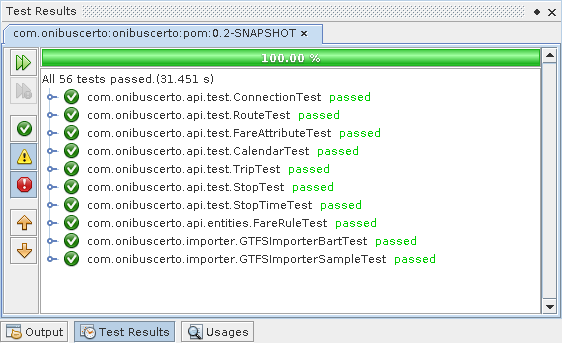
\includegraphics[width=0.6\textwidth]{./imgs/testes.png}
	\caption[Exemplo de execução dos testes]{Exemplo de execução dos testes}
	\fonte{Autoria Própria}
	\label{fig:testes}
\end{figure}

Tendo em vista que a compatibilidade do Maven com o JUnit, a popularidade e a familiaridade dos membros da equipe com este, o \emph{framework} foi escolhido como ferramenta para desenvolvimento dos casos de teste.

O uso de uma ferramenta que permita analisar qual a porcentagem de código-fonte do sistema que é coberta pelos testes escritos mostrou-se necessário.
Para tanto, a equipe optou pela ferramenta Cobertura, devido às seguintes características da mesma:

\begin{itemize}
	\item Integração com o Maven através de um \emph{plugin}.
	\item Integração com a IDE Netbeans.
	\item Geração de relatórios em HTML ou XML.
	\item Apresenta nos relatórios a porcentagem de linhas e ramificações cobertas para cada classe, pacote e para o projeto como um todo.
	\item Calcula a complexidade ciclomática de cada classe, assim como a complexidade ciclomática média para cada pacote e para o projeto.
\end{itemize}

Os relatórios gerados por esta ferramenta são de grande importância para identificar com facilidade quais partes do \emph{software} não possuem testes.
Um exemplo de relatório desta ferramenta é apresentado na Figura \ref{fig:cobertura}.

\begin{figure}[!htb]
	\centering
	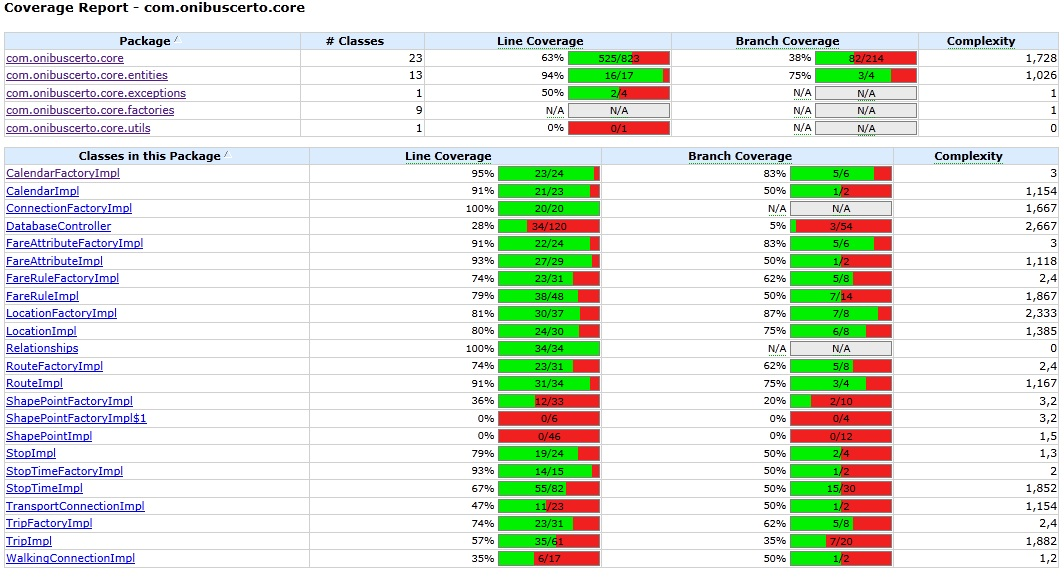
\includegraphics[width=0.8\textwidth]{./imgs/cobertura.png}
	\caption[Exemplo de relatório de cobertura de código]{Exemplo de relatório de cobertura de código}
	\fonte{Autoria Própria}
	\label{fig:cobertura}
\end{figure}

\section{Considerações}

% essa seção parece estar bem redundante, não tive tempo de reler, provavelmente tem muitas palavras repetidas que devem ser substituidas por sinônimos

O processo de desenvolvimento de \emph{software} utilizado permitiu que a equipe trabalhasse de forma distribuída, sendo necessário reunir os integrantes da mesma apenas para tomar as decisões de projeto mais importantes como definição de \emph{milestones}, discussão de interfaces entre os módulos do sistema e assegurar a qualidade do trabalho desenvolvido.
A utilização de técnicas de revisão de código por meio do uso de ferramentas específicas permitiu que a equipe discutisse detalhes da implementação remotamente, tornando os mesmos disponíveis para futuros colaboradores do projeto e reforçando a característica de um desenvolvimento distribuído.

Optar por um processo de desenvolvimento de \emph{software} que permita que os programadores trabalhem de forma distribuída mostrou-se, ao longo do processo, uma excelente opção, tendo em vista que muitas vezes os horários dos integrantes da equipe são incompatíveis.
Apesar de tornar a equipe mais eficiente como um todo e permitir que cada integrante trabalhe naquelas funcionalidades que mais lhe interessam, o processo de codificação pode prejudicar a qualidade do código.
Para resolver este problema, o uso de revisão de código e desenvolvimento orientado a estes mostrou ser de vital importância, evitando com que novos \emph{bugs} sejam introduzidos em código já testado e também evitando com que novos problemas ainda não cobertos por testes sejam criados, através de uma cuidadosa revisão.
% ^ vital importância? thanks julio!

Assim como o conjunto de práticas de desenvolvimento de software estabelecidas, as ferramentas utilizadas proporcionaram um ambiente de desenvolvimento ágil e padronizado.
O uso de um sistema de controle de versão distribuído reforçou ainda mais a característica procurada através do processo de desenvolvimento.
O uso de ferramentas como o Maven tornaram a codificação independente de IDE, permitindo que cada desenvolvedor utilize o editor de sua preferência.
Por fim, nota-se também que todas as ferramentas utilizadas reforçam o caráter de \emph{software} livre deste projeto, de forma que todos os aplicativos utilizados estão disponíveis sob licenças livres. 


%---------- Quinto Capítulo: Desenvolvimento do Software ----------
\chapter{Desenvolvimento do Software}
\label{chap:desenv}

Utilizando a metodologia e o projeto do sistema apresentados nos capítulos \ref{metod} e \ref{specs}, respectivamente, inicou-se o desenvolvimento efetivo do sistema.
Primeiramente foi criado um projeto Maven principal denominado \texttt{onibuscerto}, o qual foi dividido em quatro subprojetos: 
\begin{itemize}
	\item \texttt{onibuscerto-api}: contém classes que são de utilidade comum a todos os projetos do sistema, como classes que representam coordenadas geográficas e aquelas que compõem os objetos resposta que contém informações do caminho determinado.
	\item \texttt{onibuscerto-core}: consiste no módulo \emph{Core} definido no projeto do software (seção \ref{specs}). 
	Contém as representações das entidades originárias dos arquivos GTFS e faz a interface do sistema com o banco de dados.
	\item \texttt{onibuscerto-importer}: consiste no módulo \emph{Importer} definido no projeto do software (seção \ref{specs}).
	Responsável pela importação dos dados contidos nos arquivos GTFS para o sistema através das funcionalidades do \emph{Core}.
	\item \texttt{onibuscerto-service}: consiste nos módulos \emph{Web Service} e o Cliente \emph{Web} definidos na seção \ref{specs}.
\end{itemize}

Nas subseções a seguir serão descritos detalhes a respeito da implementação de cada subprojeto.

\section{Configuração do ambiente de desenvolvimento}

\section{onibuscerto-core}

O \emph{Core} consiste basicamente na interface do sistema com o banco de dados, contendo portanto as representações das entidades originárias dos arquivos GTFS.
Estas representações nada mais são do que \emph{wrappers}, ou seja, classes no sistema que são responsáveis pelo encapsulamento das entidades do banco de dados.
Cada uma destas classes é implementação de uma respectiva interface, e tem o intuito de referenciar um nó ou aresta do grafo armazenado.

O \emph{Core} foi organizado de tal forma que todas as suas classes de entidades possuam suas respectivas \emph{factories}.
Como já comentado, \emph{factory} consiste em uma interface com o objetivo de criação de famílias de objetos dependentes ou correlacionados.
Desta forma, toda criação de entidades é realizada através de uma \emph{factory}, centralizando este processo a somente uma classe por entidade.

Cada \emph{factory} de entidade pertencente ao arquivo GTFS é armazenada no banco de dados como um nó de referência, o qual possui uma relação para cada nó de sua respectiva entidade.
Esta organização das \emph{factories} no grafo pode ser observada na figura \ref{fig:grafoFactory}.

\begin{figure}[!htb]
	\centering
	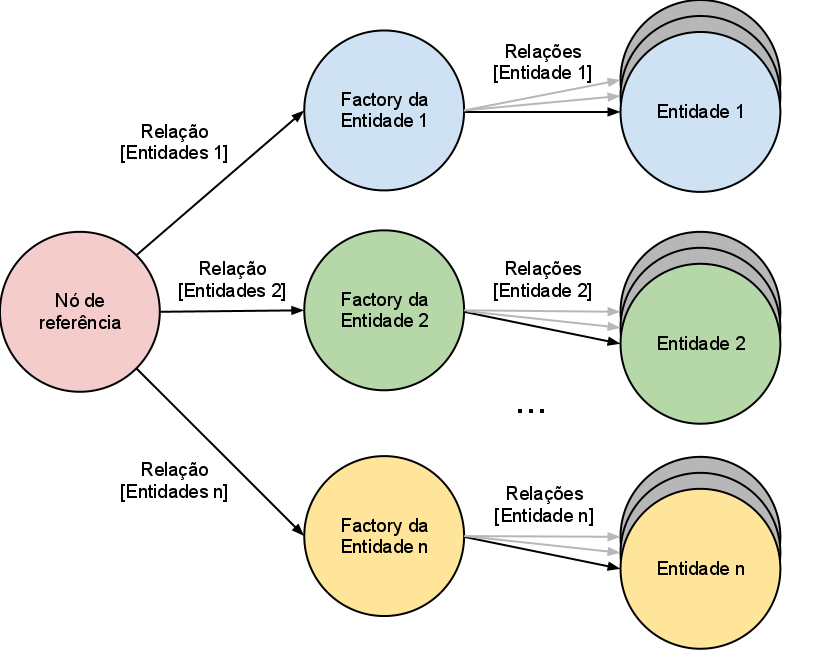
\includegraphics[width=0.7\textwidth]{./imgs/grafoFactory.png}
	\caption[Arquitetura do sistema]{Visão geral da organização das \emph{factories} do grafo.}
	\fonte{Autoria Própria}
	\label{fig:grafoFactory}
\end{figure}

A partir do nó de referência do grafo tem-se relações às \emph{factories} de todas as entidades (relação no formato [Entidades X]), sendo que estas tem relações a cada nó de seu tipo entidade (relação no formato [Entidade X]).
Com estas relações, a \emph{factory} pode ser utilizada para acessar todas as entidades do mesmo tipo, bastando percorrer o grafo.

O uso deste tipo de arquitetura torna o sistema flexível quanto ao SGBD, sendo que se necessária alguma modificação basta atualizar as \emph{factories} de acordo com o novo banco de dados. 
A seguir serão descritas todas as entidades pertencentes ao sistema, bem como a classe responsável pela interface com o banco de dados.

\subsection{Entidades}
As entidades que compõem o \emph{Core}, juntamente com suas \emph{factories}, são representadas através de interfaces e suas respectivas implementações por meio de classes no sistema. 
Desta forma toda entidade é representada no sistema através de duas interfaces e suas respectivas implementações, as quais obedecem o seguinte padrão de nomenclatura e localização (nesse contexto, \texttt{Entidade} consiste em uma representação genérica de qualquer tipo de entidade presente no sistema):
\begin{itemize}
	\item \texttt{Entidade}: interface da entidade do tipo \texttt{Entidade}.
		  Este tipo de representação é localizado no pacote \texttt{com.onibuscerto.core.entities}.
	\item \texttt{EntidadeFactory}: interface referente a \emph{factory} da \texttt{Entidade}.
		  Todas as interfaces de \emph{factories} estão localizadas no pacote \texttt{com.onibuscerto.core.factories} do subprojeto \texttt{onibuscerto-core}.
	\item \texttt{EntidadeImpl}: implementação da interface \texttt{Entidade}.
		  Todos estas implementações estão disponibilizados no pacote \texttt{com.onibuscerto.core}.
	\item \texttt{EntidadeFactoryImpl}: implementação da \emph{factory} da entidade de nome \texttt{Entidade}.
		  Estas implementações estão disponibilizadas no pacote \texttt{com.onibuscerto.core}.
\end{itemize}

Cada entidade do sistema possui suas respectivas propriedades, as quais são armazenadas no próprio nó ou aresta do grafo (dependendo de como a entidade foi armazenada no banco de dados) através de pares chave/valor, sendo estas disponíveis para futuras consultas.

%As interfaces que representam as entidades e suas \emph{factories} pertencem ao pacote \texttt{com.onibuscerto.core.entities} e %\texttt{com.onibuscerto.core.factories}, respectivamente.
%Já as implementações das mesmas estão localizadas no pacote \texttt{com.onibuscerto.core}.

A seguir serão descritos detalhes de implementação das classes que encapsulam as entidades, as quais em conjunto formam o grafo armazenado no banco de dados do sistema.

\subsubsection{Location}
Entidade responsável principalmente por representar pontos através de coordenadas geográficas, bem como suas conexões com outros pontos.
Contém basicamente em quatro atributos: 

\begin{itemize}
	\item \texttt{latitude}: latitude do ponto \emph{Location} em questão.
	\item \texttt{longitude}: longitude do ponto \emph{Location} em questão.
	\item \texttt{outgoingConnections}: coleção de conexões de entrada da \emph{Location}, representadas pela entidade do tipo \emph{Connection} (ver seção 					  \ref{conn}).
	\item \texttt{incomingConnections}: coleção de conexões de saida da \emph{Location}, também representadas pela entidade do tipo \emph{Connection} (ver seção 			  	  \ref{conn}).
\end{itemize}

A \emph{factory} assignada a esta entidade denomina-se \emph{LocationFactory} e, para este tipo de entidade, tem a funcionalidade de criar todas as entidades do tipo \emph{Location}, inclusive  suas extensões, como é o caso da entidade \emph{Stop} descrita na subseção \ref{stop}.

Esta entidade é utilizada principalmente para demarcar os pontos de origem e destino fornecidos pelo usuário que não consistem em uma parada para embarque e desembarque de passageiros.
Esta demarcação é importante para que estes pontos sejam adicionados ao grafo, desta forma contribuindo para um melhor refinamento na busca da rota com tempo de viagem mínimo.

\subsubsection{Stop}
\label{stop}
Uma \emph{Stop} consiste em uma parada de veículos para embarque e desembarque de passageiros.
Como esta também é representada por coordenadas geográficas então optou-se por implementá-la como um caso específico de uma \emph{Location}, ou seja, uma \emph{Stop} herda atributos de \emph{Location}. Desta forma, além dos atributos de \emph{Location}, cada entidade deste tipo possui os seguintes atributos:

\begin{itemize}
	\item \texttt{id}: identifica exclusivamente uma parada ou estação, porém diversos trajetos podem usar a mesma parada.
	\item \texttt{name}: nome de uma parada ou estação.
\end{itemize}

Como uma \emph{Stop} é uma especificação de \emph{Location}, utiliza-se a mesma \emph{LocationFactory}, porém neste caso com as seguintes funcionalidades:
\begin{itemize}
	\item além de criar \emph{Locations}, utiliza-se esta \emph{factory} também para criar entidades \emph{Stop} e adicioná-las a seus respectivos índices no banco 		de dados, com o intuito de facilitar futuras buscas.
	\item retornar todas as \emph{Stops} do sistema em forma de uma coleção, através de simples uma busca no grafo do sistema.
	\item retornar uma determinada \emph{Stop} com base em sua ID utilizando o índice referente a este tipo de entidade.
\end{itemize}

A informação de todas as \emph{Stops} é essencial para o funcionamento do sistema, pois sem as localizações das paradas de veículos é impossível fornecer uma rota entre dois pontos utilizando transporte público.

\subsubsection{Route}

\subsubsection{Trip}

\subsubsection{StopTime}

\subsubsection{Connection}
\label{conn}

\subsection{DatabaseController}


\section{onibuscerto-importer}

\section{onibuscerto-service}

O subprojeto \texttt{onibuscerto-service} é onde encontram-se os Servlets responsáveis por executar consultas na base de dados construída através do \emph{Importer}.
Os Servlets funcionam sob a forma de \emph{web services} e, sendo assim, todas as consultas são feitas pelos clientes através de requisições \sigla{HTTP}{Hypertext Transfer Protocol} do tipo GET ou POST.
As implementações dos Servlets residem no pacote \texttt{com.onibuscerto.service.servlets}.

Atualmente, apenas consultas que determinam a rota com o menor tempo de viagem entre duas coordenadas geográficas estão implementadas.
Estas consultas são de responsabilidade do Servlet implementado na classe \texttt{RouteServlet}.
No início do seu ciclo de vida, este é responsável por obter uma instância da classe \texttt{DatabaseController} do \emph{Core}, a qual será utilizada para acessar o banco de dados e resolver as consultas.
Em seguida, assim como um Servlet comum, este muda para um estado no qual está disponível para atender requisições dos clientes.
Por fim, ao ser destruído, o \texttt{RouteServlet} deve chamar o método \texttt{close} do \texttt{DatabaseController}, com o objetivo de fechar a conexão com o banco de dados.
O ciclo de vida completo de um Servlet é ilustrado na Figura \ref{fig:servletciclo}.

\begin{figure}[!htb]
	\centering
	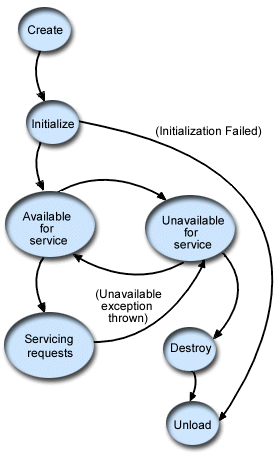
\includegraphics[width=0.4\textwidth]{./imgs/servletciclo.png}
	\caption[Ciclo de vida de um Servlet]{Ciclo de vida de um Servlet}
	\fonte{\citeonline{infocenter}}
	\label{fig:servletciclo}
\end{figure}

Enquanto o \texttt{RouteServlet} está ativo, ou seja, respondendo consultas, este recebe requisições HTTP do tipo POST com os seguintes parâmetros:
\begin{itemize}
	\item \texttt{start.latitude}: latitude do ponto de origem.
	\item \texttt{start.longitude}: longitude do ponto de origem.
	\item \texttt{end.lagitude}: lagitude do ponto de destino.
	\item \texttt{end.longitude}: longitude do ponto de destino.
	\item \texttt{departure}: horário de saída do ponto de origem, uma \emph{string} no formato \texttt{"HH:MM"}.
\end{itemize}

Ao receber estes parâmetros, o \texttt{RouteServlet} executa os seguintes passos:
\begin{enumerate}
	\item Converte as posições geográficas passadas como parâmetros para a consulta através de HTTP POST para objetos da classe \texttt{GlobalPosition}, do subprojeto \texttt{onibuscerto-api}.
	\item Cria nós no banco de dados para representar os nós de origem e destino, através da \texttt{LocationFactory}.
	\item Cria conexões do tipo \texttt{WalkingConnection} entre os recém-criados nós de origem e destino e todas as entidades do tipo \texttt{Stop} do grafo, de forma a representar os trechos que podem ser percorridos a pé pelo usuário.
	\item Executa a consulta no grafo através do método \texttt{getShortestPath} do \texttt{DatabaseController} e recebe o caminho encontrado sob a forma de um objeto do tipo \texttt{Collection<Connection>}.
	\item Converte o resultado da consulta para uma coleção de objetos da classe \texttt{QueryResponseConnection}, do subprojeto \texttt{onibuscerto-api}, ou seja, um objeto do tipo \texttt{Collection<QueryResposeConnection>}.
	\item Serializa o objeto \texttt{Collection<QueryResponseConnection>} para uma \emph{string} no formato \sigla{JSON}{JavaScript Object Notation}, o qual será finalmente enviado para o cliente do usuário.
\end{enumerate}

Tendo o funcionamento do \texttt{RouteServlet} em vista, a aplicação cliente é responsável apenas por enviar uma requisição HTTP POST para o serviço com os parâmetros no formato especificado e, por fim, interpretar os resultados retornados pelo servidor.
Uma pequena aplicação de exemplo que executa consultas no \emph{Service}, escrita em linguagem Python, é apresentada no Apêndice \ref{ape:exemplodeuso}.

\subsection{Cliente \emph{Web}}

Além dos Servlets responsáveis pelo funcionamento do \emph{web service}, o projeto \texttt{onibuscerto-service} é onde também reside o código-fonte do cliente \emph{web}.
Situado no diretório \texttt{src/main/webapp/} deste projeto, o cliente \emph{web} é composto pelos seguintes arquivos:

\begin{itemize}
	\item \texttt{index.html}: estrutura em \sigla{HTML}{Hypertext Markup Language} do \emph{layout} da página que é exibida para os usuários do cliente.
	\item \texttt{style.css}: descrição das folhas de estilo \sigla{CSS}{Cascading Style Sheets} utilizadas para renderizar o \emph{layout} da página.
	\item \texttt{script.js}: código-fonte principal do cliente, em linguagem JavaScript, responsável por todas as funcionalidades e interação do cliente \emph{web} com o service e o usuário.
\end{itemize}

Além destes arquivos, juntamente com a distribuição do cliente \emph{web} estão empacotadas as bibliotecas jQuery e jQuery UI, utilizadas para simplificar o desenvolvimento do \emph{software} em JavaScript.
Estas bibliotecas encontram-se no diretório \texttt{src/main/webapp/js/} do projeto.
As imagens utilizadas no \emph{layout} da página estão presentes no diretório \texttt{src/main/webapp/img/}.

A interface do cliente \emph{web} é composta basicamente por dois elementos: uma barra lateral e a visualização do mapa da região.
Na barra lateral está presente um formulário, através do qual o usuário pode digitar os endereços de origem e destino do caminho e o horário de partida.
Esta mesma barra é atualizada com uma descrição textual do caminho determinado pelo sistema, assim que o usuário inicia a consulta ao clicar no botão de busca.
Além disso, é possível introduzir os endereços de origem e destino clicando com o botão direito do mouse no mapa.
A figura \ref{fig:clienteweb} apresenta a interface do cliente \emph{web} com o resultado de uma consulta.

\begin{figure}[!htb]
	\centering
	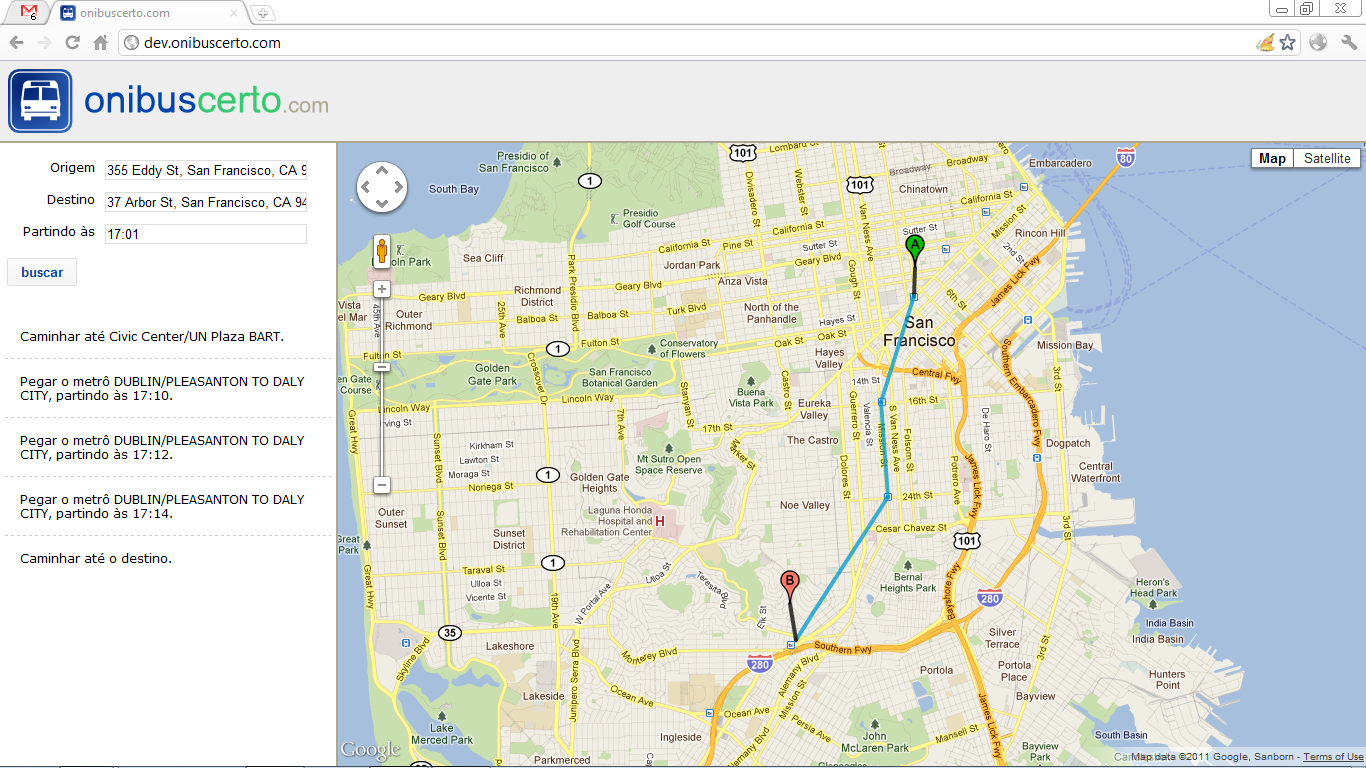
\includegraphics[width=0.9\textwidth]{./imgs/clienteweb.png}
	\caption[Interface do cliente \emph{web}]{Interface do cliente \emph{web}}
	\fonte{Autoria Própria}
	\label{fig:clienteweb}
\end{figure}

A renderização do mapa é feita através da \sigla{API}{Application Programming Interface} do Google Maps \cite{gmapsapi}, a qual permite utilizar, através de chamadas JavaScript, os mapas deste serviço de forma gratuita, contanto que o serviço que faça uso dos mapas também o seja \cite{gmapsterms}.
Esta API também conta com funcionalidades para o desenho de poli-linhas e o posicionamento de marcadores, tornando-se ideal para apresentar os resultados da consulta retornados pelo \emph{web service}.

Para realizar o processo de \emph{geocoding}, ou seja, a conversão de endereços completos como, por exemplo, ``1600 Amphitheatre Parkway, Mountain View, CA'' em coordenadas geográficas como $(37.423021, -122.083739)$, foi utilizada a API de \emph{Geocoding} do Google \cite{geocodingapi}.
De forma semelhante à API do Google Maps, esta API permite realizar este tipo de consulta diretamente através de JavaScript, sendo fornecido um endereço completo e retornando a latitude e longitude do endereço em questão.

O cliente \emph{web} pode ser utilizado simplesmente ao hospedar os arquivos do mesmo em um servidor HTTP.
No entanto, é importante notar que, caso o endereço do \emph{web service} seja diferente da página inicial do cliente \emph{web}, é necessário adaptar o endereço que é feito na requisição do mesmo, no arquivo \texttt{script.js}.
Apesar disso, ao iniciar o servidor de desenvolvimento, o cliente \emph{web} é automaticamente servido através do mesmo.
Maiores detalhes com relação à execução do \emph{software} em um ambiente de desenvolvimento estão disponíveis no Apêndice \ref{ape:guia}.

\section{Considerações}


%---------- Sexto Capítulo: Resultados ----------
\chapter{Resultados}

% TODO: resultados


\chapter{Conclusão}

Como produto do projeto em questão obteve-se uma ferramenta disponibilizada na forma de \emph{software} livre através de um serviço web, com a principal funcionalidade de auxiliar o planejamento de trajetos urbanos com o uso de transporte público.
O código-fonte do projeto inteiro está disponível livremente para o público, basta seguir os passos citados no apêndice \ref{guia}.
Desta forma, o projeto está aberto a futuras contribuições, adaptações e integrações a diversos outros sistemas, não sendo limitado somente a sua funcionalidade originalmente idelizada pela equipe.

\section{Desenvolvimento do Projeto}
%especificação
O passo inicial do projeto foi uma profunda revisão bibliográfica (localizada no capítulo \ref{fund}), como o intuito de analisar todas as tecnologias existentes e definir qual seria a mais indicada para o desenvolvimento do \emph{software}, não somente em questão de programação mas também em decisões de metodologias e técnicas de gerência de projeto utilizadas.

Decididas todas as tecnologias a serem utilizadas, o próximo passo foi o desenvolvimento da especificação do \emph{software} (capítulo \ref{specs}), a qual engloba um estudo dos requisitos do sistema e a o projeto da arquitetura a ser implementada.
Nesta fase procurou-se projetar o sistema com o intuito de modularizar ao máximo seus componentes, de tal forma que se caso necessárias modificações futuras seja rápido e fácil adapatá-lo e implementá-las.
Todos os módulos foram definidos com base nas suas respectivas funcionalidades, visando minimizar o grau de dependência entre eles. 
Isto facilita contribuições futuras ao projeto, bem como possibilitou o desenvolvimento paralelo de cada módulo, dividindo de maneira justa o trabalho entre os integrantes da equipe.

Tendo definido o que fazer e quais tecnologias utilizar, basta decidir que tipo de metodologia de desenvolvimento utilizar (capítulo \ref{metod}) para então partir para a implementação efetiva do projeto. 
A metodologia utilizada visou principalmente o trabalho em paralelo dos integrantes da equipe, já que a arquitetura do sistema possibilitou esta técnica, sendo que reuniões somente aconteceram para tomadas de decisões cruciais ao projeto, como definição de \emph{milestones} e padrões de interfaceamento entre os módulos idelizados.
Tal metodologia de desenvolvimento distribuído mostrou-se uma excelente opção ao longo do processo, já que frequentemente os horários dos integrantes da equipe se mostraram incompatíveis para reuniões periódicas.

O uso de ferramentas específicas de controle de versão e compartilhamento de código permitiu que fosse utilizada técnicas de revisão de código, as quais permitiram que os integrantes da equipe discutissem detalhes de implementação de código remotamente, sendo tais discussões disponibilizadas para futuros colaboradores. 
Estas revisões de código juntamente com desenvolvimento orientado a testes se mostraram vitais para garantir a qualidade de código, tendo em vista que o desenvolvimento distribuído torna a codificação eficiente porém sujeita a queda neste quesito.
Tais técnicas ajudaram a evitar que fossem introduzidos novos \emph{bugs} ao código já testado e que novos problemas ainda não cobertos pelos testes fosse criados.

A utilização de ferramentas como o Maven permitiram a todos os desenvolvedores utilizarem o editor de sua preferência, já que a codificação tornou-se independente da IDE utilizada.
Esta juntamente com as demais ferramentas utilizadas reforçaram o conceito de \emph{software} livre empregado ao projeto, já que todas elas estão disponíveis sob licenças livres. 

Com base na especificação do \emph{software} e na metodologia discutida, iniciou-se a fase de implementação do projeto (descrita no capítulo \ref{chap:desenv}). 
Durante tal fase procurou-se seguir de fielmente a especificação discutida no capítulo \ref{specs}, pois nesta definiu-se grande parte das decisões de arquitetura e técnicas de desenvolvimento, fazendo com que várias dificuldades de implementação fossem previstas e contornadas.
Uma destas foi a interface entre o sistema e o banco de dados, sendo que o modo como esta foi implementada tornou o sistema flexível para futuras modificações quanto ao banco de dados utilizado.

\section{Relação com Engenharia de Computação}
% TODO: Discutir a engenharia, relacionar o trabalho com as disciplinas cursadas, estágios, trabalhos
O desenvolvimento deste projeto agregou muita experiência aos membros da equipe, principalmente pela necessidade de integração de vários conceitos de diversas áreas de conhecimento estudadas ao longo do curso.
Tais conhecimentos englobam as áreas de:
\begin{itemize}
	\item \textbf{Sistemas distribuídos}: com conceitos de arquitetura cliente-servidor e controle de concorrência.
	\item \textbf{Desenvolvimento pra web}: visto que o projeto consiste basicamente em um sistema web.
	\item \textbf{Algoritmos}: sendo idealizadas adaptações de algoritmos baseados em grafos para o sistema.
	\item \textbf{Estruturas de dados}: já que diversos tipos de estruturas de dados, como vetores, grafos, listas encadeadas, foram utilizados.
	\item \textbf{Bancos de dados}: com uso de conceitos de transações no banco de dados para grafos empregado ao sistema. 
	\item \textbf{Engenharia de \emph{software}}: através do uso e adaptação de diversos conceitos, como desenvolvimento orientado a testes, uso de versionadores, 			estabelecimento de metas, entre outros.
\end{itemize}

Esta experiência é fundamental para carreira profissional de qualquer engenheiro, visto que neste projeto foram bem definidas as etapas do processo de engenhar, sendo estas necessárias para qualquer trabalho realizado. 
Tais etapas consistiram em: aquisição de base teórica, estudo do estado da arte, definição dos requisitos, projeto da arquitetura do \emph{software}, definição da metodologia utilizada, implementação efetiva do sistema e por último uma análise dos resultados alcançados. 

\section{Propostas Futuras}
% TODO: Propostas futuras
%tem que melhorar a performance do sistema com muitas requisições concorrentes
%botar shapes e fares, pegar os dados de curitiba, desenvolver um cliente android
%melhorar a interface web tanto o layout, como a disposição dos elementos as funcionalidades da interface 
%implementar consultas do tipo "quero chegar no lugar X às Y horas"
%diferentes custos pra minimizar


%---------- Referencias ----------
\bibliography{reflatex} % geracao automatica das referencias a partir do arquivo reflatex.bib


%---------- Apendices (opcionais) ----------
\apendice
\apendice
\chapter{Guia de Desenvolvimento}\label{ape:guia} % FIXME: titulo podre

Este apêndice descreve como obter o código-fonte do projeto e utilizar o \emph{software}.

% TODO

\apendice
\chapter{Exemplo de Uso do \emph{Service}}\label{ape:exemplodeuso}

Este apêndice procura fornecer um claro exemplo de como executar consultas através do componente \emph{Service} do projeto dentro de uma aplicação.
O código apresentado a seguir, em linguagem Python, executa uma consulta no serviço, decodifica o JSON do objeto resposta e, por fim, imprime o resultado na saída padrão.

Vale lembrar que, para executar este exemplo, é necessário ter instalado o interpretador da linguagem Python na versão 2.6 ou superior.

% TODO: falar que o endereço de acesso do service depende do servidor
% falar também que a URL do RouteServlet depende do especificado no arquivo web.xml do onibuscerto-service/src/main/webapp/WEB-INF

% TODO: será que esse exemplo de cliente em Python fica nessa seção mesmo?
% talvez seja melhor colocar me um anexo ou coisa parecida
% outra coisa, não sei como referenciar ele no texto, então ficou assim msm
\lstinputlisting[language=Python]{code/cliente.py}



% ---------- Anexos (opcionais) ----------
%\anexo
%\chapter{Nome do Anexo}

%Use o comando {\ttfamily \textbackslash anexo} e depois comandos {\ttfamily \textbackslash chapter\{\}}
%para gerar t\'itulos de anexos.


% --------- Lista de siglas --------
%\textbf{* Observa\c{c}\~oes:} a lista de siglas nao realiza a ordenacao das siglas em ordem alfabetica
% Em breve isso sera implementado, enquanto isso:
%\textbf{Sugest\~ao:} crie outro arquivo .tex para siglas e utilize o comando \sigla{sigla}{descri\c{c}\~ao}.
%Para incluir este arquivo no final do arquivo, utilize o comando \input{arquivo.tex}.
%Assim, Todas as siglas serao geradas na ultima pagina. Entao, devera excluir a ultima pagina da versao final do arquivo
% PDF do seu documento.


%-------- Citacoes ---------
% - Utilize o comando \citeonline{...} para citacoes com o seguinte formato: Autor et al. (2011).
% Este tipo de formato eh utilizado no comeco do paragrafo. P.ex.: \citeonline{autor2011}

% - Utilize o comando \cite{...} para citacoeses no meio ou final do paragrafo. P.ex.: \cite{autor2011}



%-------- Titulos com nomes cientificos (titulo, capitulos e secoes) ----------
% Regra para escrita de nomes cientificos:
% Os nomes devem ser escritos em italico, 
%a primeira letra do primeiro nome deve ser em maiusculo e o restante em minusculo (inclusive a primeira letra do segundo nome).
% VEJA os exemplos abaixo.
% 
% 1) voce nao quer que a secao fique com uppercase (caixa alta) automaticamente:
%\section[nouppercase]{\MakeUppercase{Estudo dos efeitos da radiacao ultravioleta C e TFD em celulas de} {\textit{Saccharomyces boulardii}}
%
% 2) por padrao os cases (maiusculas/minuscula) sao ajustados automaticamente, voce nao precisa usar makeuppercase e afins.
% \section{Introducao} % a introducao sera posta no texto como INTRODUCAO, automaticamente, como a norma indica.


\end{document}
